In this chapter we develop a \emph{Picard iteration} aiming to solve the \MA equation. To the author's knowledge this is the first try to apply the \emph{Picard linearisation} on the \MA equation. 
We first motivate and derive the Picard iteration and its discretisation.
Afterwards we compare the method with the classical Netwon's method and the $C^0$ penalty method presented in the previous chapter (cf. Section \ref{sec: Brenner method}). We try to transfer results on the penalty method to the newly derived Picard iteration method. 
In the last section first numerical results are presented. Since the Picard iteration does not perform well on a first example we discuss improvements of the newly derived method.


\section{A Picard Iteration for the \MA equation} \label{sec: motivation picard iteration}
For quasilinear PDEs (cf. Definition \ref{def: categories of PDEs}) such as the convection equation $\nabla \cdot (A(u) \nabla u ) = f$ it is common to determine the solution via a fixed point iteration \cite{Deblois1997,LL1995,MNK2009}. The key aspect is a decoupling of the coefficient matrix $A(u)$ and $\nabla u$. Hence, one solves iteratively for $i\in \N$ the equations
\[
	\nabla \cdot (A(u^{i} )\nabla u^{i+1}) = f. %  \quad \text{      and      }\quad \nabla \cdot (A(u^{i+1}) \nabla u^{i}) = f, \text{ respectively}.
\] 
This kind of linearisation is also called \emph{Picard linearisation} method and is very favoured to linearise the convection term in the Navier-Stokes equations.

In this spirit we aim to decouple of the derivatives in the strongly nonlinear \MA such that the decoupled PDEs are linear. 

Before we start, we slightly change notation: Differing to the preceding sections we denote the elements of $\Omega \subset \R^2$ by  $(x,y)^t$. To shorten and facilitate terms we refer to their partial derivatives with subscripts as for example $\dxy{x}{y} u = u_{xy}$.
Thus, the two-dimensional \MA equation \eqref{eq: MA eq} states
\begin{align}
 \mydet{D^2 u} &= f \nonumber \\
 	\Leftrightarrow \qquad  \dyy u{x}  \dyy u{y}  -\dyx u {x}{y} \dyx u {y}{x} &= f. \label{eq:mongeAmpere detForm}
\end{align}

First, we multiply \eqref{eq:mongeAmpere detForm} by $2$ and expand the left-hand side
\begin{align}
% 	2\dyy u {x} \dyy u {y}-2\dyx u {x}{y} \dyx u{y}{x}  &= 2 f \\
 	\dyy u {x} \dyy u {y}+\dyy u {x} \dyy u {y} -\dyx u {x}{y} \dyx u{y}{x} -\dyx u {x}{y} \dyx u{y}{x} &=2 f. 
\end{align}

Formally decoupling into the two functions $v = u ,w = u$ and reordering terms we have
\begin{align}
	w_{yy} v_{xx}- w_{xy} v_{yx} - w_{yx} v_{xy} +w_{xx} v_{yy} = 2f. \label{eq:decoupled PDE start}
\end{align}
Rewriting this by matrix Frobenius product (cf. Definition \ref{def: frobenius product}) leads to
\begin{align}
 \begin{pmatrix} w_{yy} & -w_{xy}  \\ -w_{yx} & w_{xx} \end{pmatrix}: \begin{pmatrix} v_{xx} & v_{yx}  \\  v_{xy} & v_{yy} \end{pmatrix} = 2f.
\end{align}
We observe that the left matrix is the cofactor matrix of the Hessian (cf. Definition \ref{def: cof matrix}) and the right one is the Hessian itself and hence
\begin{align}
		\mycof {D^2 w }:D^2 v  = 2f. \label{eq:short formula}
\end{align}
Note that this derivation of decoupling of $v$ and $w$ is chosen for it is very intuitive. Alternatively \eqref{eq:short formula} can be derived directly from the identity $\mycof {D^2 u }:D^2 u  = d \mydet{D^2 u}$ stated in Lemma \ref{la: rel det cofactor}.

Substituting the identity of Lemma \ref{la: An application of the divergernce product rule} and multiplying with -1 we find
\begin{align}
	- \nabla \cdot \left( \mycof{ D^2 w} \nabla v \right)  = -2f.  \label{eq:decoupled PDE}
\end{align}

For a fixed $w$ the left-hand side now is linear in $v$ opposed to the strong nonlinearity in $u$ in the original PDE. It is a Generalised Poisson equation in $v$ as we have defined in Definition \ref{def: General Poisson Problem}. 
Furthermore as it is easy to see in \eqref{eq:decoupled PDE start} the left-hand side is symmetric in $v$ and $w$. Thus, it is natural to examine a sequence of PDEs where alternating either $v$ or $w$ is fixed. 

Adding the Dirichlet boundary condition we obtain the Picard iteration
\begin{align}
	\begin{split}
	- \nabla \cdot \left( \mycof{ D^2 u^i} \nabla u^{i+1} \right)  &= -2f  \text{ in } \Omega \\
		u^{i+1} &= g \textnormal{ on } \partial \Omega.
	\label{eq:fixed point iteration}
	\end{split}
\end{align}

Taking a closer look at the derivation of \eqref{eq:decoupled PDE} we see only rearrangements and the smoothness of $w$ were used. Hence, for any smooth solution $u$ the \MA equation can also be written as
\begin{align}
- \nabla \cdot \left( \mycof{ D^2 u} \nabla u \right)  = -2f.  \label{eq: analytical fixed point iteration}
\end{align}
This also implies that every solution of a \MA problem is a fixed point of the Picard iteration. It remains to test if the Picard iteration converges to its fixed point and hence yields an approximation of the solution of the \MA equation. 


\section{Discretisation of a Picard Iteration Step}\label{sec: SIPG MA}
Since every iteration \eqref{eq:fixed point iteration} states a Generalised Poisson equation we can apply the derived SIPG method of Section \ref{sec: SIPG} directly: Given $u^i_h\in \mathcal P^k_h$ find $u^{i+1}_h \in \mathcal P^k_h$ satisfying
\begin{align}
 &\myIntX {\Omega} {\nabla v_h \cdot \cof(D_h^2 u_h^{i}) \nabla u_h^{i+1}}  \nonumber\\
 & -\sum\limits_{e \in \edges}\myIntS e { \jump {v_h \average { \cof(D_h^2 u^{i}) \nabla u_h^{i+1}} }}
 - \sum\limits_{e \in \edges}\myIntS e { \jump {u_h^{i+1} \average{ \cof(D^2 u_h^{i}) \nabla v_h} }} \nonumber\\  
 &  +\sum\limits_{e \in \edgesi} \myIntS e { \frac \sigma {|e|} \jump {v_h}  \jump {u_h^{i+1}}}\nonumber\\
    =& - 2 \myIntX {\Omega} {v_h f}
    	 				-\sum\limits_{e \in \edgesb}\myIntS e {g \cof(D^2 u_h^{i}) \nabla v_h \cdot n }
    	 				+\sum\limits_{e \in \edgesb} \myIntS e { \frac \sigma {|e|} v_h g}    \qquad \forall v_h \in  \mathcal P^k_h.
    	\label{eq: sipg iteration}
\end{align}

Now that we derived a new iterated DG method to solve the \MA equation we compare \eqref{eq: sipg iteration} to Newton's method and the method introduced in Section \ref{sec: Brenner method}. 

\section{Comparison with Newton's method}

Let us apply Newton's method directly on the analytical form of the \MA equation (cf. \eqref{eq: MA eq}).
Let $F$ be the \MA operator, i.e. 
\[
	F(u) = \mydet{D^2 u} -f.
\]
To apply Newton's method on $F(u) =0$ we have to find $u^{i+1}$ satisfying
\begin{align}
	DF[u^i](u^{i+1}-u^i) = -F[u^i]
\end{align}
where $DF[u]$ denotes the G\^ateaux derivative of $F$ at $u$. We derived the G\^ateaux derivative $DF[u] v = \mycof{D^2 u}:D^2v$ already in Theorem \ref{thm: linearisation}, leading us to the Newton iteration
\begin{align}
	\mycof{D^2 u^i}:D^2\left(u^{i+1}-u^i\right) &= -\mydet{D^2 u^i}+f \nonumber \\
	\Leftrightarrow \qquad \qquad  \mycof{D^2 u^i}:D^2(u^{i+1}) &= -\mydet{D^2 u^i} +f  +\mycof{D^2 u^i}:D^2(u^i). \label{eq: Newton iteration pre}
\end{align}

For further rearrangements we recall the identities from Lemma \ref{la: rel det cofactor} and Lemma \ref{la: An application of the divergernce product rule}, i.e. 
\begin{align}
	\nabla \cdot \left( \mycof {D^2 u } \nabla v \right)
	\stackrel{La.\ref{la: An application of the divergernce product rule}}=\mycof{D^2 u}:D^2u
	\stackrel{La.\ref{la: rel det cofactor}}=2 \mydet{D^2u}. \label{eq: cof identities}
\end{align}

Similar to the derivation of the Picard iteration in Section \ref{sec: motivation picard iteration} we can apply \eqref{eq: cof identities} to rewrite \eqref{eq: Newton iteration pre} and we have the problem
\begin{align}
	\nabla \cdot \left( \cof(D^2 u^i) \nabla u^{i+1} \right) &= -\mydet {D^2u^i} +f+\mycof{D^2 u^i}:D^2(u^i)  \textnormal{ in } \Omega,  \label{eq: Newton iteration}\\
	u^{i+1} &= g \textnormal{ on } \partial \Omega .
\end{align}

Hence, considering the fact of \eqref{eq: cof identities} and $\detHess {u^i} \approx f$ we can interpret the Picard method as a variant of Newton's method. 

In \cite{Awanou2014} Awanou analysed an iteration process similar to just presented Newton iteration:
\begin{align}
	\nabla \cdot \left( \cof(D^2 u^0) \nabla u^{i+1} \right) &= \nabla \cdot \left( \cof(D^2 u^0) \nabla u^{i} \right) + f - \operatorname{det} (D^2u^i) \textnormal{ in } \Omega,  \label{eq: Awanout eq}\\
	u^{i+1} &= g \textnormal{ on } \partial \Omega.
\end{align}
Note that term $\mycof{D^2 u^i}:D^2(u^i)$ in \eqref{eq: Newton iteration} equals to $\nabla \cdot \left( \cof(D^2 u^i) \nabla u^{i} \right)$ by \eqref{eq: cof identities}. Thus, Awanou's formulation is the Newton iteration with fixed diffusion matrices.\\
For this analytical formulation he proves convergence to the \MA solution $u$ under the assumption that the initial guess $u^0$ is sufficient close to $u$. Unfortunately, his analysis is not applicable to the Picard iteration as he relies on the fact that the left-hand side of \eqref{eq: Awanout eq} does not alter for different $u^i$.\\
In an earlier work \cite{Awanou2010} Awanou examined a discrete version of a vanishing moment method, herein he mentioned a method he calls Newton's method \cite[(1.3)]{Awanou2010}: Find $u_h^{i+1}\in V_h$ such that for all $v_h \in V_h \cap H^1_0 (\Omega)$
\[
	\myIntX {\Omega} {[\mycof{ D^2 u_h^i} Du_h^{i+1}] \cdot Dv_h} 
	= -	\myIntX{\Omega} {f v_h} 
		+ \frac 1 2 \myIntX{\Omega} {[\mycof{ D^2 u_h^i} Du_h^{i}] \cdot Dv_h} \;  \label{eq: Awanout eq2}.
\]
And indeed this is the variational form of \eqref{eq: Newton iteration} using the identity in \eqref{eq: cof identities} and integration by parts.
He chooses the trial space to consist of piecewise polynomials contained in $C^1(\Omega)$ and claims without further explanation that this ansatz breaks down for problems with non-smooth solutions\cite[Introduction]{Awanou2010}, in his numerical results he cites test \ref{test sqrt} as an example where Newton's method diverges \cite[Section 4.4]{Awanou2010}.

%\begin{align}
%	&\myInt_\Omega \cofHess {u^i} \nabla (u^{i+1}-u^i) \nabla v - \sum_{e \in \edgesb} \myIntS e { \cofHess {u^i} \nabla (u^{i+1}-u^i) \cdot \mathbf n \; v \nonumber \\
%	&- \sum_{e \in \edgesb} \myIntS e { \cofHess {u^i} \nabla v \cdot \mathbf n (u^{i+1}-u^i) + \sigma \sum_{e \in \edgesb} \frac 1 {|e|} \myIntS e { v (u^{i+1}-u^i)\nonumber \\
%	=&-\myInt_\Omega \left(f - \detHess{u^i)}\right) v  
%			- \sum_{e \in \edgesi} \myIntS e { \jump { \average{\cofHess {u^i}} \nabla {u^i} } v \nonumber \\
%&	- \sum_{e \in \edgesb} \myIntS e { \cofHess {u^i} \nabla v \cdot \mathbf n \; (u^i-g) - \sigma \sum_{e \in \edgesb} \frac 1 {|e|} \myIntS e { v (u^{i}-g) \label{eq: a newton step Brenner}
%\end{align}
%To compare both linearisations we first reorder and remove cancelling terms in \eqref{eq: a newton step Brenner}.
%\begin{align}
%	&\myInt_\Omega \cofHess {u^i} \nabla u^{i+1} \nabla v \\
%	&- \sum_{e \in \edgesb} \myIntS e { \cofHess {u^i} \nabla u^{i+1} \cdot \mathbf n \; v 
%		- \sum_{e \in \edgesb} \myIntS e { \cofHess {u^i} \nabla v \cdot \mathbf n \; u^{i+1} \\
%	&+\sigma \sum_{e \in \edgesb} \frac 1 {|e|} \myIntS e { v u^{i+1}\\
%	=
%	&-\myInt_\Omega \left(f - \detHess{u^i)}\right) v \\
%	&- \sum_{e \in \edgesi} \myIntS e { \jump { \average{\cofHess {u^i}} \nabla {u^i} } v 
%		+ \sum_{e \in \edgesb} \myIntS e { \cofHess {u^i} \nabla {u^i} \cdot \mathbf n \; v\\
%	&- 2\sum_{e \in \edgesb} \myIntS e { \cofHess {u^i} \nabla v \cdot \mathbf n \; {u^i}
%		+ \sum_{e \in \edgesb} \myIntS e { \cofHess {u^i} \nabla v \cdot \mathbf n \; g \\
%	&+\sigma \sum_{e \in \edgesb} \frac 1 {|e|} \myIntS e { v g \label{eq: ordered newton step Brenner}
%\end{align}

\section{Analysis of the DG Method} \label{sec: DG analysis}
This section compares the newly derived method with the $C^0$ penalty method by Brenner et al. \cite{BGN+2011}, already presented in Section \ref{sec: Brenner method}, on a analytical basis. In particular we examine how we can transfer the analysis of the penalty method to the Picard iteration.

\subsection{Comparison with a $C^0$ Penalty method}\label{subsec: comparison brenner}
Brenner et al. emphasis that it is important that the linearisation of a \MA method is a consistent and stable discretisation of the linearisation of the \MA equation, namely $\nabla \cdot \left( \mycof {D^2 u } \nabla (v) \right)$ \cite[Remark 2.2]{BGN+2011}.
Therefore we first compare the linearisation of the Picard iteration with the linearisation of the method introduced by Brenner et al. \cite{BGN+2011}.

Let us consider again the linearisation of the finite element method mentioned in Section \ref{sec: Brenner method}, namely the mapping $L^B_u:H^2(\Omega; \triang) \rightarrow [H^2(\Omega; \triang) \cap H^1(\Omega)]'$ (cf. \eqref{eq: var of linearisation}) given by
\begin{align}
\bilin {L^B_{u} w} v
	=&\myIntX  \Omega { (\cofHess{ u}\nabla w) \cdot \nabla v}
		- \sum_{e \in \edgesb} \myIntS e { (\cofHess{u}\nabla w) \cdot \mathbf n \; v} \nonumber \\
		&-  \sum_{e \in \edgesb} \myIntS e { (\cofHess{u}\nabla v) \cdot \mathbf n \; w} 
		+ \sigma \sum_{e \in \edgesb} \frac 1 {|e|} \myIntS e { v w}.
		\label{eq: linearisation brenner}
\end{align}


Looking at the Picard iteration in \eqref{eq:fixed point iteration} we see that we aim to solve the discretised linearisation of the \MA equation at the point $u^i$ in every step.\\
Let $V$ be $H^2(\Omega; \triang) \cap L^2(\Omega)$ and $L_u: V \rightarrow V'$ denote the linear mapping describing the left-hand side of the SIPG method (cf. \eqref{eq: sipg iteration}) to perform an iteration step, i.e.
\begin{align}
	\bilin {L_u w} v =
 &\myIntX  \Omega { \nabla v \cdot \cof(D_h^2 u) \nabla w } \nonumber\\
 & -\sum\limits_{e \in \edges}\myIntS e { \jump {v \average { \cof(D_h^2 u) \nabla w} }}
 - \sum\limits_{e \in \edges}\myIntS e { \jump {w \average{ \cof(D^2 u) \nabla v} }} \nonumber\\  
 & +\sum\limits_{e \in \bigEps} \myIntS e { \frac \sigma {|e|} \jump {v}  \jump {w}}. \label{eq: linearisation our}
\end{align}
Comparing now \eqref{eq: linearisation our} with \eqref{eq: linearisation brenner} we notice that they are equal except for the interior edge integrals. But this difference is only due to the different choice of ansatz spaces: While in \cite{BGN+2011} Brenner et al. use $C^0$ elements, the Picard iteration is based on $DG$ elements. For the continuous ansatz functions all function jumps across interior edges vanish and hence all interior edge integrals equal to zero.

Consider $u\in H^s(\Omega)$ for $s>3$ to be the convex solution of the \MA problem. Brenner et al. formulated a nonlinear finite element method with the goal that its linearisation at the solution $u$ is given by \eqref{eq: linearisation brenner}. In other words their penalty method can be formulated by a mapping $F^B:H^3(\Omega; \triang) \rightarrow [H^2(\Omega; \triang) \cap H^1(\Omega)]'$ satisfying
 \begin{align}
 	F^B(u +w ) = L^B_u w + R^Bw \label{eq: add brenner method}
 \end{align}
 with a (nonlinear) mapping $R^B:H^3(\Omega; \triang) \rightarrow [H^2(\Omega; \triang) \cap H^1(\Omega)]'$. 
% They compute $R^B$ to be given by
% \begin{align}
% 	\bilin {R^B w} v 
% 	= & - \myInt_\Omega \detHessH{w} v dx 
% 		+ \sum_{e \in \edgesi} \jump {\average{\cofHessH{w}} \nabla w} v ds \nonumber \\
% 		&- \sum_{e\in \edgesb} \myIntS e { \cofHessH{w} \nabla v \cdot \mathbf{n} \; w ds 
% \end{align}.
% 
We want to derive a similar identity for the Picard iteration. 

For the rest of the analysis, we consider a convex and polyhedral domain $\Omega\subset \R^2$ and $f,g$ such that the \MA problem has a unique convex solution $u \in H^s(\Omega)$ with $s\geq 2$. 

Note that from now on $u$ denotes a fixed function. While Brenner et al. only linearise $F$ at the point $u$ the Picard method linearises at the last step's solution. Thus, $L_u^B$ defined in \eqref{eq: linearisation brenner} has always the same parameter $u$, namely the exact solution, whereas the parameter $u$ in the definition of $L_u$ (cf. \eqref{eq: linearisation our}) varies. 

To derive results on the Picard iteration, we follow the argumentative structure Brenner et al. used to show convergence of their method in \cite{BGN+2011}. At first, we introduce the functional $R_u \in V'$ for the right-hand side of the SIPG method defined by
\begin{align}
\bilin {-R_u} v = - 2 \myIntX  \Omega {v f}
-\sum\limits_{e \in \edgesb}\myIntS e { g \cofHessH{u} \nabla v \cdot \mathbf n }
+\sum\limits_{e \in \edgesb} \myIntS e { \frac \sigma {|e|} v g}. \label{eq: definition R}
\end{align}
The desired discretised Picard iteration then states: Find $u^{i+1}_h \in V_h$ such that
\begin{align}
\bilin {L_{u^i_h} w_h} {v_h} =  \bilin {-R_{u^i_h}} {v_h}   \qquad \forall v_h \in V_h. \label{eq: fixed point functional}
\end{align}
Formulating this as an operator equation yields: Find $u_h^{i+1} \in V_h$ being a root of the function $F:V \rightarrow V'$ defined by
\begin{align}
 {Fw} =  L_{u^i_h} w + R_{u^i_h}  \qquad \text{ for } w \in V. \label{eq: definition F}
\end{align}



Thus we have the identity 
\begin{align}
	F(u+w) = L_{u^i_h} (u+w) + R_{u^i_h} = L_{u^i_h} u +L_{u^i_h}w + R_{u^i_h} = Fu + L_{u^i_h}w. \label{eq: add our method}
\end{align}

Let us compare \eqref{eq: add brenner method} with \eqref{eq: add our method}: We have already seen the commonality of both methods, they base on the same linearisation and thereby gain the permutability between linearisation and discretisation. 
But there are also two major differences: While the right-hand side of \eqref{eq: add brenner method} contains a nonlinear mapping $R^B$, \eqref{eq: add our method} contains the additional term $Fu$. \\
Note that \eqref{eq: add brenner method} also be written as 
 \begin{align*}
 F^B(u +w ) = F^B u + L^B_u w + R^Bw,
 \end{align*}
since the exact \MA solution is a root of the finite element method operator. 
Hence, the distinction between both approaches can be characterised: While the first one reproduces the nonlinearity of the \MA equation with a nonlinear term, the second ansatz replaces parts of the nonlinear terms of the equation by an approximation and thus, trades nonlinearity for consistency errors.

\subsection{Consistency Estimates}

To measure the error in the second derivative we introduce a new quantity. Let $\epsilonTwoZeroArg:V \rightarrow \R$ be defined by
\[
	\epsilonTwo{v} := \max{ \LTwonorm{\hess v}}{ \sup_{e \in \edges} \LTwonormE{\average{\hess v}}}.
\]	

The following lemma shows $\epsilonTwo{\cdot}$ is not only a measure for the Hessian, but also for the cofactor of the Hessian.
\begin{lemma} \label{la: epsilon cof hess equal}
	For any convex $v \in V$ it holds
	\[
		\epsilonTwo{v} = \max{ \LTwonorm{\cofHessH v}}{ \sup_{e \in \edges} \LTwonormE{\average{\cofHessH{v}}}}
	\]
\end{lemma}
\begin{proof}
	We have for a positive definite matrix $A$ that 
	\begin{align*}
	\LTwonorm{A} =  \sup_{v \in L^2(\Omega), \LTwonorm{v}=1} \myIntX \Omega {v^t A^t A v} = \lambda^2,
	\end{align*}
	where $\lambda$ is the largest eigenvalue of $A$. Since for every $w \in V$ the eigenvalues of $\cofHessH{w}$ and $\hess{w}$ coincide on every $T \in \triang$ we obtain 
	\begin{align}
	\LTwonormT{\cofHessH{w}} = \LTwonormT{\hess{w}} \qquad \forall T \in \triang.\label{eq: equality norm}
	\end{align}
	Furthermore using the definition of the average (cf. Definition \ref{def: edge operators}) and that $\cofHessH{w}$ and $\hess{w}$ are linear in $w$ for all $w \in V$ we find
	\begin{align}
	\LTwonormE{\average {\cofHessH{w}}} 
	=& \LTwonormE{\frac 1 2 {\cofHessH{(w^+ + w^-)}}} \nonumber\\
	=& \LTwonormE{\frac 1 2 {\hess{(w^+ + w^-)}}} 
	= \LTwonormE{\average {\hess{w}}} \qquad \forall e \in \edges. \label{eq: equality norm average}
	\end{align}
	\phantom{blub}
\end{proof}

Let for $w \in V$ the mapping $L_{w,h}:V_h \rightarrow V_h'$ be the restriction from $L_w$ to $V_h$. All further analysis is based on the following lemma.
\begin{lemma}[Stability] \label{la: stability L}
	Suppose $w \in V$ to be convex. Then 
	\begin{align}
		\HMinusOneDnorm{L_{w}v} \leq \epsilonTwo{w} \eNorm{v} \qquad \forall v \in V.
	\end{align}
	Further, for a penalty parameter $\sigma $ sufficiently large $L_{w,h}: V_h \rightarrow V_h'$ is invertible and satisfies
	\begin{align}
		\eNorm{L_{w,h}^{-1} r_h} \leq C \HMinusOneDnorm{r_h} \qquad \forall r_h \in V_h'.
	\end{align}
	$C$ denotes a positive constant independent on $h$ and $r_h$. 
\end{lemma}
\begin{proof}
	Since for convex $w$ the cofactor matrix is always positive definite the claim follows from the proof of Theorem \ref{thm: SIPG stability}.
\end{proof}

Note that this means $F$ defined in \eqref{eq: definition F} has a unique solution in $V_h$ as $R$ is constant in $w$.

For further analysis we want to examine the dependence of $L_w$ on the parameter $w$.
\begin{lemma}\label{la: L dependence parameter}
	For $w_1, w_2 \in V$ holds
	\[
		\HMinusOneDnorm{L_{w_1} v - L_{w_2} v} \leq \epsilonTwo{w_1 - w_2} \eNorm{v} \qquad \forall v \in V,
	\]
\end{lemma}
\begin{proof}
	Let $w_1, w_2, v$ be in $V$. For any $\varphi_h \in V_h$ we have by the definition of $L$ in \eqref{eq: linearisation our} and by linearity
	\begin{align}
		\bilin{L_{w_1}v- L_{w_2} v} {\varphi_h} =  
			&\myIntX  \Omega { \nabla \varphi_h \cdot \cofHessH{(w_1-w_2)} \nabla v}  \nonumber\\
			& -\sum\limits_{e \in \edges}\myIntS e { \jump {\varphi_h \average { \cofHessH{(w_1-w_2)} \nabla v} }} \nonumber \\
			& - \sum\limits_{e \in \edges}\myIntS e { \jump {v \average{ \cofHessH{(w_1-w_2)} \nabla \varphi_h} }}. \label{eq: diff linear}
	\end{align}
	As already done in the proof of Theorem \ref{thm: SIPG stability} we use the Cauchy-Schwarz inequality and the discrete Cauchy-Schwarz inequality on every summand and obtain that $\bilin{L_{w_1}v- L_{w_2} v} {\varphi_h}$ is smaller than
	\begin{align*}
%		\eqref{eq: diff linear}%\bilin{L_{w_1}v- L_{w_2} v} {\varphi_h} 
%		\leq
		& \LTwonorm{\nabla \varphi_h} \LTwonorm{\cofHessH{(w_1 -w_2)}} \LTwonorm {\nabla v} \nonumber \\
			&+ \left( \sum_{e \in \edges} \frac {\sigma}{|e|}\LTwonormE{\jump {\varphi_h}}^2 \right)^{\frac 1 2}
			   \left( \sum_{e \in \edges} \frac {|e|} \sigma\LTwonormE{\average{\cofHessH{(w_1-w_2} \nabla v}}^2 \right)^{\frac 1 2} \\
			&+ \left( \sum_{e \in \edges} \frac {\sigma}{|e|}\LTwonormE{\jump v}^2 \right)^{\frac 1 2}
			\left( \sum_{e \in \edges} \frac {|e|} \sigma\LTwonormE{\average{\cofHessH{(w_1-w_2} \nabla \varphi_h}}^2 \right)^{\frac 1 2}
	\end{align*}
	and hence with Lemma \ref{la: epsilon cof hess equal}
	\begin{align*}
		\bilin{L_{w_1}v- L_{w_2} v} {\varphi_h}
		\leq& \epsilonTwo{w_1 - w_2} \\
			&\times 
			\left( \LTwonorm{\nabla \varphi_h} \LTwonorm {\nabla v} 
				\phantom{\left( \sum_{e \in \edges} \frac {|e|} \sigma\LTwonormE{\average{\nabla \varphi_h}}^2 \right)^{\frac 1 2}}
			 \right.\nonumber \\
			&\phantom{\times \;\;\;}+ \left( \sum_{e \in \edges} \frac {\sigma}{|e|}\LTwonormE{\jump {\varphi_h}}^2 \right)^{\frac 1 2}
			\left( \sum_{e \in \edges} \frac {|e|} \sigma\LTwonormE{\average{\nabla v}}^2 \right)^{\frac 1 2} \\
			&\phantom {\times \;\;\;}+ \left( \sum_{e \in \edges} \frac {\sigma}{|e|}\LTwonormE{\jump v}^2 \right)^{\frac 1 2}
			\left. \left( \sum_{e \in \edges} \frac {|e|} \sigma\LTwonormE{\average{\nabla \varphi_h}}^2 \right)^{\frac 1 2} \right).
	\end{align*}
	Using now the discrete Cauchy-Schwarz inequality on the whole term yields
	\begin{align*}
		\bilin{L_{w_1}v- L_{w_2} v} {\varphi_h} 
		\leq& \epsilonTwo{w_1 - w_2} \\
		  & \times 
			\left( 
				\LTwonorm{\nabla \varphi}^2
					+ \sum\limits_{e \in \edges} \frac {\sigma} {|e|}\LTwonormE{\jump {\varphi}}^2
					+ \sum\limits_{e \in \edges} \frac {|e|} \sigma \LTwonormE{\average{\nabla \varphi}}^2
				\right)^{\frac 1 2} \nonumber \\
			&\times
			\left( 
				\LTwonorm{\nabla v}^2
					+\sum\limits_{e \in \edges} \frac {\sigma}{|e|}\LTwonormE{\jump {v}}^2
					+ \sum\limits_{e \in \edges} \frac {|e|} \sigma \LTwonormE{\average{\nabla v}}^2
			\right) ^{\frac 1 2} \nonumber \\
			\leq & \epsilonTwo{w_1 - w_2} \eNorm \varphi \eNorm v.
	\end{align*}
	The result follows then with Definition \ref{def: h-1 seminorm}.
%	Since the eigenvalues of $\cofHessH{(w_1-w_2}$ and $\hess{(w_1-w_2)}$ coincide their $L^2$ norm also coincides. Hence, by this and the discrete Cauchy-Schwarz inequality it follows
%	\begin{align}
%		\eqref{eq: diff linear 2} %\bilin{L_{w_1}v- L_{w_2} v} {\varphi_h} 
%		\leq& \LTwonorm{\nabla \varphi_h} \LTwonorm{\hess{(w_1 -w_2)}} \LTwonorm {\nabla v} \nonumber \\
%			&+ \LInftynorm{\jump {\varphi_h}} 
%				\left(\sum_{e \in \edges} \LTwonormE{\average{\hess{(w_1-w_2}}}^2 \right)^{\frac 1 2} 
%				\left(\sum_{e \in \edges} \LTwonormE{\average{\nabla v}}^2 \right)^{\frac 1 2} \nonumber \\
%			&+ 	\left(\sum_{e \in \edges} \LTwonormE{\jump v}^2 \right)^{\frac 1 2} 
%				\left(\sum_{e \in \edges} \LTwonormE{\average{\hess{(w_1-w_2}}}^2 \right)^{\frac 1 2} 
%				\LInftynorm{\average{\nabla \varphi_h}}. \label{eq: estimate diff L}
%	\end{align}
%	By the definition of jump and average it is clear that 
%	\[
%		\LInftynorm{\jump {\varphi_h}} = \LInftynorm{\varphi_h}\text{ and }\LInftynorm{\average{\nabla \varphi_h}}= \LInftynorm{\nabla \varphi_h}
%	\]
%	hold. Further we can estimate the $L^\infty$ norm using the discrete Sobolev inequality (\todo{discrete sobolev}) and we find
%	\begin{align}
%		\LInftynorm{\average {\nabla \varphi_h}} \leq C (1+|\ln h|^{\frac 1 2}) \LTwonorm{\nabla \varphi_h} \leq C (1+|\ln h|^{\frac 1 2}) \eNorm{\nabla \varphi_h}, \label{eq: estimate average phi}
%	\end{align}
%	and
%	\begin{align}
%		\LInftynorm{\jump {\varphi_h}} \leq C (1+|\ln h|^{\frac 1 2}) \LTwonorm{\varphi_h}. \label{eq: first estimate jump phi}
%	\end{align}
%	To further estimate \eqref{eq: first estimate jump phi} we apply the inverse estimate from Lemma \ref{la: inverse estimate} and the Poincar\'e inequality (\todo{poincare inequality}) and obtain
%	\begin{align}
%		\LTwonorm{\varphi_h} = \sum_{T \in \triang} \LTwonormT{\varphi_h} \leq C h \sum_{T \in \triang} \HOnenormT{\varphi_h} \leq C h \sum_{T \in \triang} \singleNorm{\varphi_h}_{H^1(T)} \leq Ch \eNorm{\varphi_h} \label{eq: estimate phi}
%	\end{align}
%	By \eqref{eq: estimate average phi}, \eqref{eq: first estimate jump phi} and \eqref{eq: estimate phi} and $h<1$, we have
%	\begin{align}
%		\maxTriple{\LTwonorm{\nabla \varphi}}{\LInftynorm{\jump{\varphi_h}}}{\LInftynorm{\average{\nabla \varphi_h}}} \leq C (1+|\ln h|^{\frac 1 2}) \eNorm{\varphi_h}
%	\end{align} 
%	and hence by \eqref{eq: estimate diff L}
%	\begin{align}
%		\bilin{L_{w_1}v- L_{w_2} v} {\varphi_h} 
%		\leq& C (1+|\ln h|^{\frac 1 2})\eNorm{\varphi} 
%			\left[ 
%				\LTwonorm{\hess{(w_1 -w_2)}} \LTwonorm {\nabla v} \nonumber \right.\\
%				&+ 	\left(\sum_{e \in \edges} \LTwonormE{\average{\hess{(w_1-w_2}}}^2 \right)^{\frac 1 2} 
%					\left(\sum_{e \in \edges} \LTwonormE{\average{\nabla v}}^2 \right)^{\frac 1 2} \nonumber \\
%				&+ 	\left(\sum_{e \in \edges} \LTwonormE{\jump v}^2 \right)^{\frac 1 2} 
%				\left. \left(\sum_{e \in \edges} \LTwonormE{\average{\hess{(w_1-w_2}}}^2 \right)^{\frac 1 2} 
%			\right] \label{eq: difference estimate number two}
%	\end{align}
%\todo{brackets}	
%	Using the discrete Cauchy-Schwarz inequality we find
%	\begin{align}
%	\bilin{L_{w_1}v- L_{w_2} v} {\varphi_h} 
%		\leq& C (1+|\ln h|^{\frac 1 2})\eNorm{\varphi} 
%		\nonumber \\
%		&\times
%			\left(
%				\LTwonorm{\hess{(w_1 -w_2)}}^2 
%				+ 2\sum_{e \in \edges} \LTwonormE{\average{\hess{(w_1-w_2}}}^2
%			\right)^{\frac 1 2} \nonumber \\
%	   	&\times
%			\left(
%			\LTwonorm{\nabla v}^2 
%			+ \sum_{e \in \edges} \frac {|e|}\sigma \LTwonormE{\average{\nabla v}}^2
%			+\sum_{e \in \edges} \frac \sigma {|e|}\LTwonormE{\jump {v}}^2
%			\right)^{\frac 1 2} \nonumber \\
%		\leq& C (1+|\ln h|^{\frac 1 2})\eNorm{\varphi} 	\epsilonTwo{{(w_1-w_2)}} \eNorm{v}
%	\end{align}
% \phantom{blub}
\end{proof}


Now we are able to establish an estimate of the consistency error of $Fu$.
\begin{theorem}[Consistency Error of $Fu$] \label{la: consistency error F}
	There holds
	\begin{align*}
	\HMinusOneDnorm{Fu} \leq& C (\eNorm{u}+1)\epsilonTwo{u-u_h^i},
	\end{align*}
	where $C$ is a positive constant that depends on the mesh, $g$ and $u^i_h$, but not on $h$ and $u$. 
\end{theorem}
\begin{proof}
	We have for $v \in V_h$
	\begin{align}
	%		\bilin{Fu} v = \myIntX  \Omega {
	\HMinusOneDnorm{Fu} =& \HMinusOneDnorm{ L_{u^i_h}u + R_{u^i_h}} \nonumber\\
	\leq& \HMinusOneDnorm{ L_{u^i_h}u - L_u u} + \HMinusOneDnorm{ L_{u}u + R_u} + \HMinusOneDnorm{ -R_u + R_{u^i_h}}. \label{eq: Fu first estimate}
	\end{align}	
	The exact solution $u$ is a fixed point of $- \nabla \cdot \left( \mycof{ D^2 u^i} \nabla u^{i+1} \right)  = -2f$ (cf. \eqref{eq:fixed point iteration}). The mappings $L_w$ and $R_w$ were defined to formulate the SIPG method for this equation (cf. \eqref{eq: fixed point functional}). Thus, we obtain
	\begin{align}
	L_{u} u + R_u = 0. \label{eq: right solution L+U}
	\end{align}
	By the definition of $R$ in \eqref{eq: definition R} and the Cauchy-Schwarz inequality we find for any $v \in V_h$ 
	\begin{align}
	\bilin {R_u - R_{u^i_h}} v 
	=& \sum_{e \in \edgesb} \myIntX \Omega {g \cofHessH{(u-u_h^i)} \nabla v \cdot \mathbf n }\nonumber \\
	\leq& \LInftynormPOm{g}
		\sum_{e \in \edgesb} \LTwonormE{ \cofHessH{(u-u_h^i)} \nabla v }^2 \nonumber \\
	\leq& \LInftynormPOm{g}
		\left( \sum_{e \in \edgesb} \frac {|e|} \sigma \LTwonormE{ \cofHessH{(u-u_h^i)}}^2  \right)^{\frac 1 2}
		\left( \sum_{e \in \edgesb} \frac \sigma {|e|} \LTwonormE{\nabla v }^2  \right)^{\frac 1 2}. \label{eq: R first estimate}
	\end{align}
	Using again \eqref{eq: equality norm}, namely that the $L^2$ norm of a matrix and its cofactor matrix coincide, as well as the standard combination of the trace estimate from Lemma \ref{la: trace estimate} and the inverse estimate from Lemma \ref{la: inverse estimate}\footnote{for more detailed steps of the combination of trace and inverse estimate see the proof of Lemma \ref{la: equivalence energy norm}} we find
	\begin{align}
	\sum_{e \in \edgesb} \frac 1 {|e|} \LTwonormE{ \cofHessH{(u-u_h^i)}}^2 
	\leq C \sum_{T \in \triang} \LTwonormT{\hess{(u-u_h^i)}}^2.
	\end{align}
	Combining this with \eqref{eq: R first estimate} yields
	\begin{align*}
	\bilin {R_u - R_{u^i_h}} v \leq C \eNorm{v} \epsilonTwo{u-u_h^i}
	\end{align*}
	and hence 
	\begin{align}
	\HMinusOneDnorm{R_u - R_{u^i_h}} \leq C \epsilonTwo{u-u_h^i}. \label{eq: contraction R}
	\end{align}
	The consistency error estimate then follows from \eqref{eq: Fu first estimate}, Lemma \ref{la: L dependence parameter}, \eqref{eq: right solution L+U} and \eqref{eq: contraction R}.
\end{proof}

This result is very important to understand the derived method. It states that the consistency error depends linearly on the error $\epsilonTwo{u-u^i_h}$. That means the method is only consistent if $\epsilonTwo{u-u^i_h}$ depends linearly on $h^l$ for a $l \geq 1$. Otherwise the consistency error is not controllable and in particular the introduced method is not consistent.

\subsection{Error estimates}
Now we want to transfer the argument structure given by Brenner et al. to derive error estimates. So, analogously to their definition in \cite[(3.1)]{BGN+2011} we define the operator $\mathcal M: V \rightarrow V_h$ by
\begin{align}
	\mathcal M = L_{u,h}^{-1}(L_{u} - F).
\end{align}
Let $\mathcal M_h:V_h \rightarrow V_h$ be its restriction to $V_h$. Clearly, $\mathcal M_h$ reduces to 
\begin{align}
\mathcal M = id_h - L_{u,h}^{-1}F.
\end{align}
Since $L_{u,h}$ is a isomorphism every fixed point of $\mathcal M_h$ is also a root of $F$ and hence a fixed point to the Picard iteration.

We want to derive a contraction property as well as a mapping property to apply Banach's fixed point theorem. If we are able to show that $\M_h$ restricted to an arbitrary small set is a self-mapping we can locate the fixed point with arbitrary precision. Like Brenner et al. \cite[(3.3)]{BGN+2011} we choose this set to be a small ball centred around $u_{c,h}\in V_h$, where
\[
u_{c,h} = L_{u,h}^{-1} L_u u.
\]

By \eqref{eq: add our method} for all $w \in V$
\begin{align}
	\mathcal M w &= L_{u,h}^{-1}(L_u w - Fw) \nonumber\\
				 &= L_{u,h}^{-1}(L_u w - F(u+w-u)) \nonumber\\
				 &= L_{u,h}^{-1}(L_u w - Fu - L_{u^i_h} (w-u)) \nonumber\\
				 &=  L_{u,h}^{-1}(L_u w - L_{u^i_h} w + L_{u^i_h}u - L_u u + L_u u - Fu) \nonumber\\
				 & = u_{c,h} + L_{u,h}^{-1}(L_u w - L_{u^i_h} w + L_{u^i_h}u - L_u u - Fu) \label{eq: expand M}
 \end{align}
and hence for $w_1, w_2 \in V$
\begin{align*}
	\eNorm{\mathcal M w_1 - \mathcal M w_2} =& \eNorm{L_{u,h}^{-1}(L_u (w_1-w_2) - L_{u^i_h} (w_1-w_2))}.
\end{align*}
Applying Lemma \ref{la: stability L} and Lemma \ref{la: L dependence parameter} yields the following contraction result which is motivated by \cite[Lemma 3.4]{BGN+2011}.
\begin{lemma}[Contraction property of $\mathcal{M}$] \label{la: contraction property M}
	For any $w_1, w_2 \in V$ it holds for a positive constant $C$ independent on $h$
\begin{align*}
	\HOneDnorm{\mathcal M w_1 - \mathcal M w_2}	\leq C \epsilonTwo{u - u^i_h} \eNorm{w_1 - w_2}. \label{eq: estimate M}
\end{align*}
\end{lemma}
It is easy to see that the contraction property of $\mathcal{M}$ depends strongly on the approximation quality of the last step's solution. %If this estimation is sharp it also means that 

Before we prove the self-mapping property, we want justify the choice of $u_{c,h}$. Therefore we show $u_{c,h}$ is close to the exact \MA solution.

\begin{lemma}\label{la: difference u uch}
	The distance between the exact solution $u$ and $u_{c,h}$ is mainly determined by the approximation properties of $V_h$, namely
	\[
		\eNorm{u-u_{c,h}} \leq C \inf_{v_h \in V_h} \eNorm{u-v_h},
	\]
	where $C>1$ denotes a constant independent on $h$, but dependent on $u$.
\end{lemma}
\begin{proof}
	For any $v_h \in V_h$ holds applying the definition of $u_{c,h}$ and both statements given in Lemma \ref{la: stability L}
	\begin{align}
		\eNorm{u-u_{c,h}} \leq& \eNorm{u- v_h} + \eNorm{ v_h- L_{u,h}^{-1}L_u u} \nonumber \\
			=& \eNorm{u- v_h} + \eNorm{L_{u,h}^{-1}L_{u,h} v_h- L_{u,h}^{-1}L_u u} \nonumber \\
			\leq& \eNorm{u- v_h} + C \HMinusOneDnorm{L_{u,h} v_h-  L_u u} \nonumber \\
			\leq& \eNorm{u- v_h} + C \epsilonTwo{u}\eNorm{v_h -u} \nonumber
	\end{align}
	Since $v_h \in V_h$ was arbitrary the desired estimate follows.
\end{proof}

Let us now derive an estimate for the image of a small ball centred at $u_{c,h}$ inspired by the estimate \cite[Lemma 3.6]{BGN+2011}.
\begin{lemma}[Mapping Property of $\M$] \label{la: mapping property of M}
	Let 
	\[
		\mathbb B_\rho(u_{c,h}):=\{v_h \in V_h: \eNorm{v_h - u_{c,h}} \leq \rho\}
	\]
	denote a small ball in $V_h$ centred at $u_{c,h}$. 
	Then, there holds for any $v \in \mathbb B_\rho(u_{c,h})$
	\[
		\eNorm{u_{c,h} - \M_h v} \leq C \epsilonTwo{u - u^i_h} (\rho+ \inf_{v_h \in V_h} \eNorm{u-v_h}+1),
	\]
	where $C$ is a positive constant independent on $h$, but dependent on $u$.
\end{lemma}
\begin{proof}
By \eqref{eq: expand M} we have for any $w \in V$
	\begin{align}
		\eNorm{u_{c,h} - \M_h w} = \eNorm{L_{u,h}^{-1}(L_u w - L_{u^i_h} w + L_{u^i_h}u - L_u u - Fu)}
	\end{align}
	and hence using Lemma \ref{la: stability L} and \ref{la: L dependence parameter}
	\begin{align*}
		\eNorm{u_{c,h} - \M_h w} 
		\leq& C\HMinusOneDnorm{(L_u w - L_{u^i_h} w + L_{u^i_h} u- L_u u - Fu)} \nonumber\\
		\leq& C\HMinusOneDnorm{(L_u (w-u) - L_{u^i_h} (w-u) - Fu)} \nonumber\\
				\leq& C \epsilonTwo{u - u^i_h} \eNorm{w-u} +\HMinusOneDnorm{Fu}.
	\end{align*}
	Using the result in Lemma \ref{la: consistency error F} we obtain
	\begin{align*}
		\eNorm{u_{c,h} - \M_h w} \leq& C \epsilonTwo{u - u^i_h} (\eNorm{w-u}+\eNorm{u} +1)\nonumber \\
		\leq & C \epsilonTwo{u - u^i_h} (\eNorm{w-u}+1).
	\end{align*}
	Consider now $v_h \in \mathbb B_\rho(u_{c,h})$, by the triangle inequality we find 
	\begin{align}
		\eNorm{u_{c,h} - \M_h v} 
			\leq& C \epsilonTwo{u - u^i_h} (\eNorm{v_h-u_{c,h}}+ \eNorm{u_{c,h}-u} +1) \nonumber \\
			\leq& C \epsilonTwo{u - u^i_h} (\rho+ \eNorm{u_{c,h}-u} +1)			
	\end{align}
Using the estimate of Lemma \ref{la: difference u uch} implies the claimed estimate.
\end{proof}

This result is inspired by Lemma 3.6 in \cite{BGN+2011}. Once again, we observe the differences of the two methods: While the statement in this Lemma relies on the previous consistency estimates, the estimate derived by Brenner et al. depends on the contraction property of the nonlinear part $R^B$ from \eqref{eq: add brenner method}. 

%which states 
%\begin{align}
%	\eNorm{u^B_{c,h} - \mathcal{M}^B_h v} \leq C_1 h^{-2} (1+|\ln h|^{\frac 1 2} ) \left(\rho^2+C_2 h^{2(l-1)} \norm u_{H^l(\Omega)}^2 \right) \label{eq: estimate Brenner}
%\end{align}
%Note that $u^B_{c,h}$ and $\mathcal{M}^B_h v$ are analogously to $u_{c,h}$ and $\mathcal{M}_h$ defined using the $L^B$ and $R^B$ from \ref{eq: add brenner method}. We observe that 
%%

Now we are able to combine the preceding results and thereby derive an estimate as in the main theorem of \cite{BGN+2011}.
\begin{theorem}\label{main result}
	Given a sufficiently large $\sigma$ and $u_h^i$ sufficiently close to the exact solution, there exists a solution $u_h$ to the penalty method \eqref{eq: fixed point functional} satisfying
	\begin{align}
		\eNorm{u-u_h} \leq C h^{s-1}, \label{eq: error estimate}
	\end{align}
	where $0 \leq s \leq \min\{k+1, t\}$ for $u$ contained in $H^t(\Omega)$. Hereby $C$ denotes a positive constant depending on the mesh, $g$, $\sigma$, $u^i_h$, and $u$, but not on $h$.\\
	Furthermore if there exists $C^*$ independent on $h$ such that
	\begin{align}
		\epsilonTwo{u-u_h^i} \leq C^* h^{s}, \label{eq: estimate error}
	\end{align}
	then there exist a $h^*> 0$ such that $u_h^i$ fulfils the requirements to apply \eqref{eq: error estimate} for all $h > h^*$.
	
\end{theorem}
\begin{proof}
	Fix $h$ and take
	\begin{align}
		\rho_0:= h^{s-1} \norm{u}_{H^{s}(\Omega)}. \label{eq: definition rho0}
	\end{align}
	
	Define 
	\begin{align}
		\tau_1 &= 2 C_1 \epsilonTwo{u-u_h^i}, \label{eq: tau1}\\
		\tau_2 & = 2 C_2 \epsilonTwo{u-u_h^i}, \label{eq: tau2}\\
		\tau_3 & = C_2 \epsilonTwo{u-u_h^i} \left(\inf_{v_h \in V_h} \eNorm{u-v_h}+1\right) 2 \rho_0^{-1} \label{eq: tau3},
	\end{align}
	where $C_1$ is the constant of Lemma \ref{la: contraction property M} and $C_2$ the constant of Lemma \ref{la: mapping property of M}. 
	
	Let $u_h^i$ suffice
	\begin{align}
		%\max
		\delta := \maxTriple {\tau_1} {\tau_2} {\tau_3}< 1,
	\end{align}
	Thereby it follows from \eqref{eq: tau1} that $\M$ fulfils the contraction property stated in Lemma \ref{la: contraction property M} with the constant $\tau_1\leq \delta<1$.
	
	Lemma \ref{la: mapping property of M} implies for any $v_h \in \mathbb{B}_{\rho_0}(u_{c,h})$
	 \[
	 	\eNorm{u_{c,h} - \M_h v_h} \leq 
	 		C_2 \epsilonTwo{u - u^i_h} (\rho_0+ \inf_{v_h \in V_h} \eNorm{u-v_h}+1) 
	 \]
	By \eqref{eq: tau2} we have 
	 \[
	 	\eNorm{u_{c,h} - \M_h v_h} \leq 
	 		\frac \delta 2 \rho_0 
	 			+ C_2  \epsilonTwo{u - u^i_h} \left( \inf_{v_h \in V_h} \eNorm{u-v_h}+1\right)
	 \]
	 and then by \eqref{eq: tau3} we obtain
	 \begin{align}
	 	\eNorm{u_{c,h} - \M_h v_h} \leq 
	 		\frac \delta 2 \rho_0 
	 		+ \frac {\rho_0} 2  < \rho_0. \label{eq: self mapping M}
	 \end{align} 
	 
	 Now we fulfil all requirements to apply Banach's fixed point theorem: $\mathbb{B}_{\rho_0}(u_{c,h}), $ is a closed subset of the Banach space $(V_h, \eNorm{\cdot})$, and $\mathcal M_h$ is a contraction mapping on $ \mathbb{B}_{\rho_0}(u_{c,h})$. Hence, the theorem yields the existence of a unique fixed point $u_h$ of $\M_h$ in $\mathbb B_{\rho_0}$.
	 Moreover, by Lemma \ref{la: difference u uch} it holds
	 \begin{align}
	 	\eNorm{u-u_h} \leq \eNorm{u-u_{c,h}} + \eNorm{u_{c,h} - u_h} \leq C \inf_{v_h \in V_h} \eNorm{u-v_h} +\rho_0 
	\end{align}
	\eqref{eq: error estimate} then follows by the approximation property given in Lemma \ref{la: approximation properties} and scaling.
	
	Given $\epsilonTwo{u-u_h^i} \leq h^{s+1} \norm{u}_H^s(\Omega)$ we find using the definitions of $\rho_0$ and $\tau_3$ (cf. \eqref{eq: definition rho0} and \eqref{eq: tau3})
	\begin{align*}
		\tau_3  \leq C h^{s} \left(h^{s-1} \norm{u}_{H^s(\Omega)}+1\right) h^{-s+1} \norm{u}_{H^{s}(\Omega)}^{-1} \xrightarrow{h \rightarrow 0}  0.
	\end{align*}
	Since analogously $\tau_1, \tau_2 \xrightarrow[]{h\rightarrow 0} 0$ holds there exist $h^*$ such that their maximum, namely $\delta$, is smaller than 1.
\end{proof}
	
Note that $\mathcal P^k_h$ for $u \in H^t(\Omega)$ has the approximation property  (cf. Lemma \ref{la: approximation properties})
\begin{align}
	\inf_{v \in V_h} \sum_{T \in \triang} \singleNorm{u-v_h}_{H^2(T)} \leq h^{l-2} \singleNorm{u}_{H^l(\Omega)}, \label{eq: approx hess}
\end{align}
where $l = \min\{k+1,t\}$. $\singleNorm{u-u^i_h}_{H^2(\Omega)} = \LTwonorm{\hess {(u-u^i_h)}}$ influences $\epsilonTwo{u-u^i_h}$ and thus, Theorem \ref{main result} yields even for a reliable approximation of $u$ no satisfying result on the Picard Iteration. Furthermore, if we have a guess that fulfils \eqref{eq: estimate error} this theorem does not ensure $u_h$ is a better approximation to $u$ than $u^i_h$. 

The analogue result for the method of Brenner et al. \cite[Theorem 3.1]{BGN+2011} yields optimal convergence results, but they depend on the property that $l$ defined as in \eqref{eq: approx hess} is strictly greater than $3$ to control the mapping property of $\mathcal M$. However, we depend on the error in the second derivatives, i.e. $\epsilonTwo{u-u_h^i}$ to control this mapping property. The problem is that derived mapping property in Lemma \ref{la: mapping property of M} is not sufficient to imitate the results of Brenner et al. as it does not decrease linearly with a power of $h$.

Unfortunately, later numerical results suggest that this formulation of a Picard Iteration do not converge to the \MA solution.	
	


%After this analysis it is not clear how the Picard iteration practically behaves. The next section addresses some first numerical results of the Picard iteration and first obstacles when solving simple problems.  
\section{Challenges for the Picard iterations}
Reviewing existing DG methods for the \MA equation we learned some issues we have to pay attention to, while examining the performances of the Picard iteration. The next subsections treat the most challenging points.
At the beginning there always is the question of a starting point $u_h^0$.
\subsection{Initial Guess}\label{sec: initial guess}
Just as most methods for the \MA equation the fixed point iteration requires an initial guess. Two approaches are very favoured in the literature.
In \cite[Remark 2.1]{DG2006a} has been shown a strong connection between the \MA problem, and  the following Poisson problem
\begin{align}
	\begin{split}
	\triangledown u &= \sqrt{2f} \text{ in } \Omega, \\ 
	u &= g \text{ on }\partial \Omega.
	\end{split}\label{eq: start sqrt_f}
\end{align}
An advantage of this approach is the compliance of boundary conditions.

Alternatively a nested iteration can be utilised. On the coarsest level with a grid width $h_1$ one chooses any convex function as initial guess $u^0_{h_1}$. Often the polynomial $\frac 1 2 ({x_1^2} + {x_2^2}) $ is taken for it is convex and has a low degree. For finer triangulations $\mathcal{T}_{h_{l}}$ the solution of the previously computed solution $u_{h_{l-1}}$is taken as a starting point. Of course both approaches can be combined using the Poisson solution of \eqref{eq: start sqrt_f} on the coarsest grid whereas later taking quasi-interpolants.\\
The second approach is preferable as it takes into account that the robustness of the method may decrease for finer meshes.

Now we are able to perform the Picard iteration on some simple example cases.
\subsection{An additional Penalty Parameter} \label{subsec: add penalty param}
At the beginning the SIPG method is implemented exactly as stated in Section \ref{sec: SIPG MA}. The polynomial degree $k$ of the ansatz and trial space $\mathcal V_h^k$ is taken to be two.
The solution of \eqref{eq: start sqrt_f} serves as an initial guess, the penalty parameter $\sigma$ is chosen to be 30 and the domain $\Omega$ to be the unit square $[0,1]^2$.

For first numerical results we consider the rather simple equation
\begin{align}
	\mydet {D^2 u} &= 1 \text{ in } \Omega, \\ 
	u &= \frac 1 2 (x_1^2 + x_2^2 )\text{ on }\partial \Omega,
\end{align}
with the exact classical solution $\frac 1 2 (x_1^2 + x_2^2 )$. 

\begin{figure}[H]
	\centering
	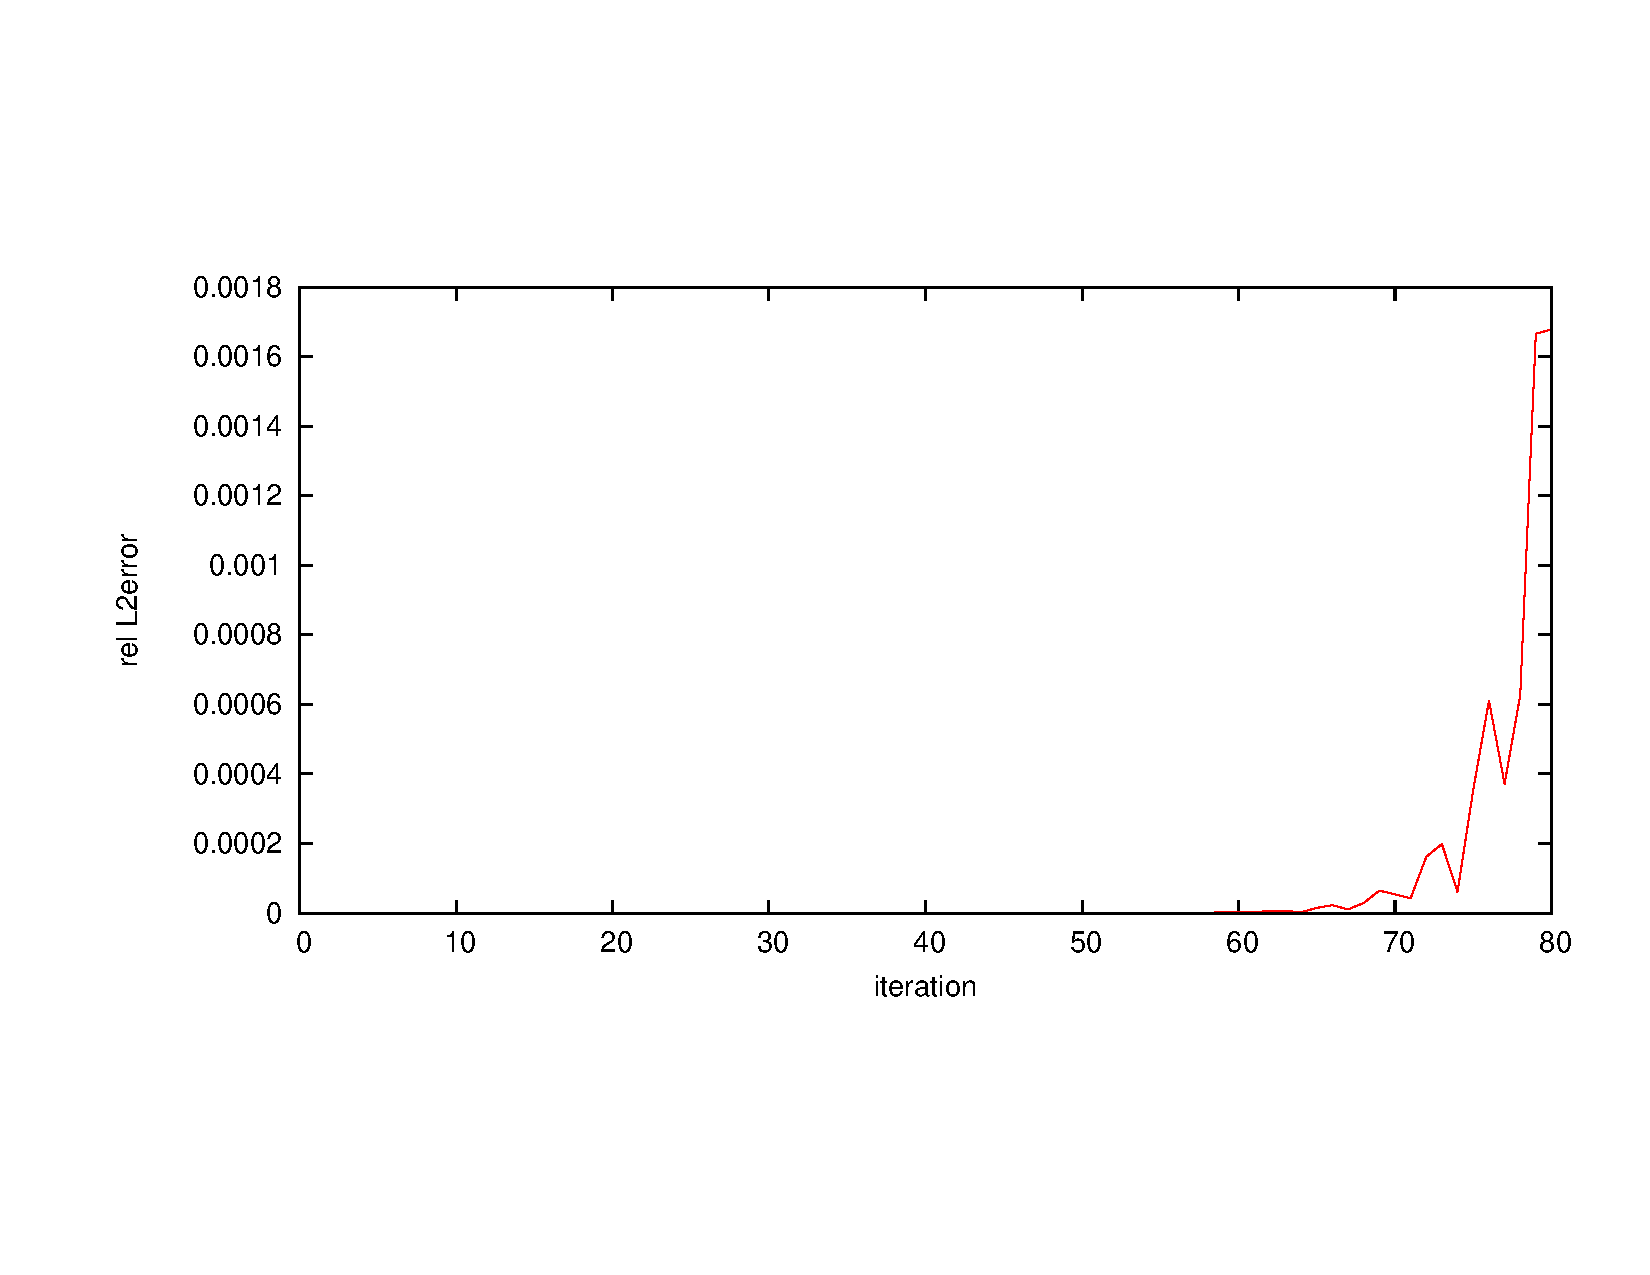
\includegraphics[trim = 2cm 4cm 1cm 4cm, scale =0.5]{plots/consisctency_first_try.pdf}
	\caption{Relative $L^2$ error on a uniform grid with $h=\frac 1 2$}
	\label{fig: consisctency_first_try}
\end{figure}
However, even for this rather simple example the implementation shows inconsistencies: Given the exact solution which is already contained in $V_h$ as starting point the $L^2$ error increases, as shown in Figure \ref{fig: consisctency_first_try}.

Examining the plots of solutions $u^i_h$ shortly before the method diverges it catches the eye that they have developed some sharp edges although the initial function and the solution are absolutely smooth. In particular the sharp edges of the solution coincide with the edges of the finite element grid. A visual inspection suggest that these solution $u^i_h$ are $C^0$ continuous, but lack higher regularity.

An idea is to force more regularity on the first derivative and thus, implicitly obtain a more smooth solution. This suits to the improvement Neilan introduced for low degrees \cite[Section 5]{Neilan2014} which is also described at the end of Section \ref{subsec: disrete Hessian}. His proposed correction terms vanish as the gradient jump across internal edges tends to zero.
Hence, we add the same normal derivatives penalty term 
\begin{align}
	\sum_{e \in \edgesi} \sigma_g |e |\myIntS e {\jump{ \nabla u} \jump {\nabla v}} \label{eq: grad penalty term}
\end{align}
to the left-hand side of \eqref{eq: sipg iteration}.
This avoids variational crimes by interior jumps of derivatives along interior edges of the triangulation. We implicitly assume that the desired solution is contained in $H^2(\Omega)$, it is not yet clear how this term behaves for a less regular solution.
With the new penalisation of the gradient we observe that an modified implementation is consistent with the previous example. The same test as at the beginning of this section was carried out with the choice $\sigma_g$ equal to $\sigma=30$ and now the $L^2$ errors stayed for 200 iterations numerically zero.
%\todo{Noelle gluecklich machen querschnitt}

Nevertheless, starting over with the initial guess from \eqref{eq: start sqrt_f} the method is unstable and diverges. But the results yet are very remarkable. As shown in Figure \ref{fig: oscillation} the error is oscillating while diverging  to infinity.
\begin{figure}[H]
	\centering
	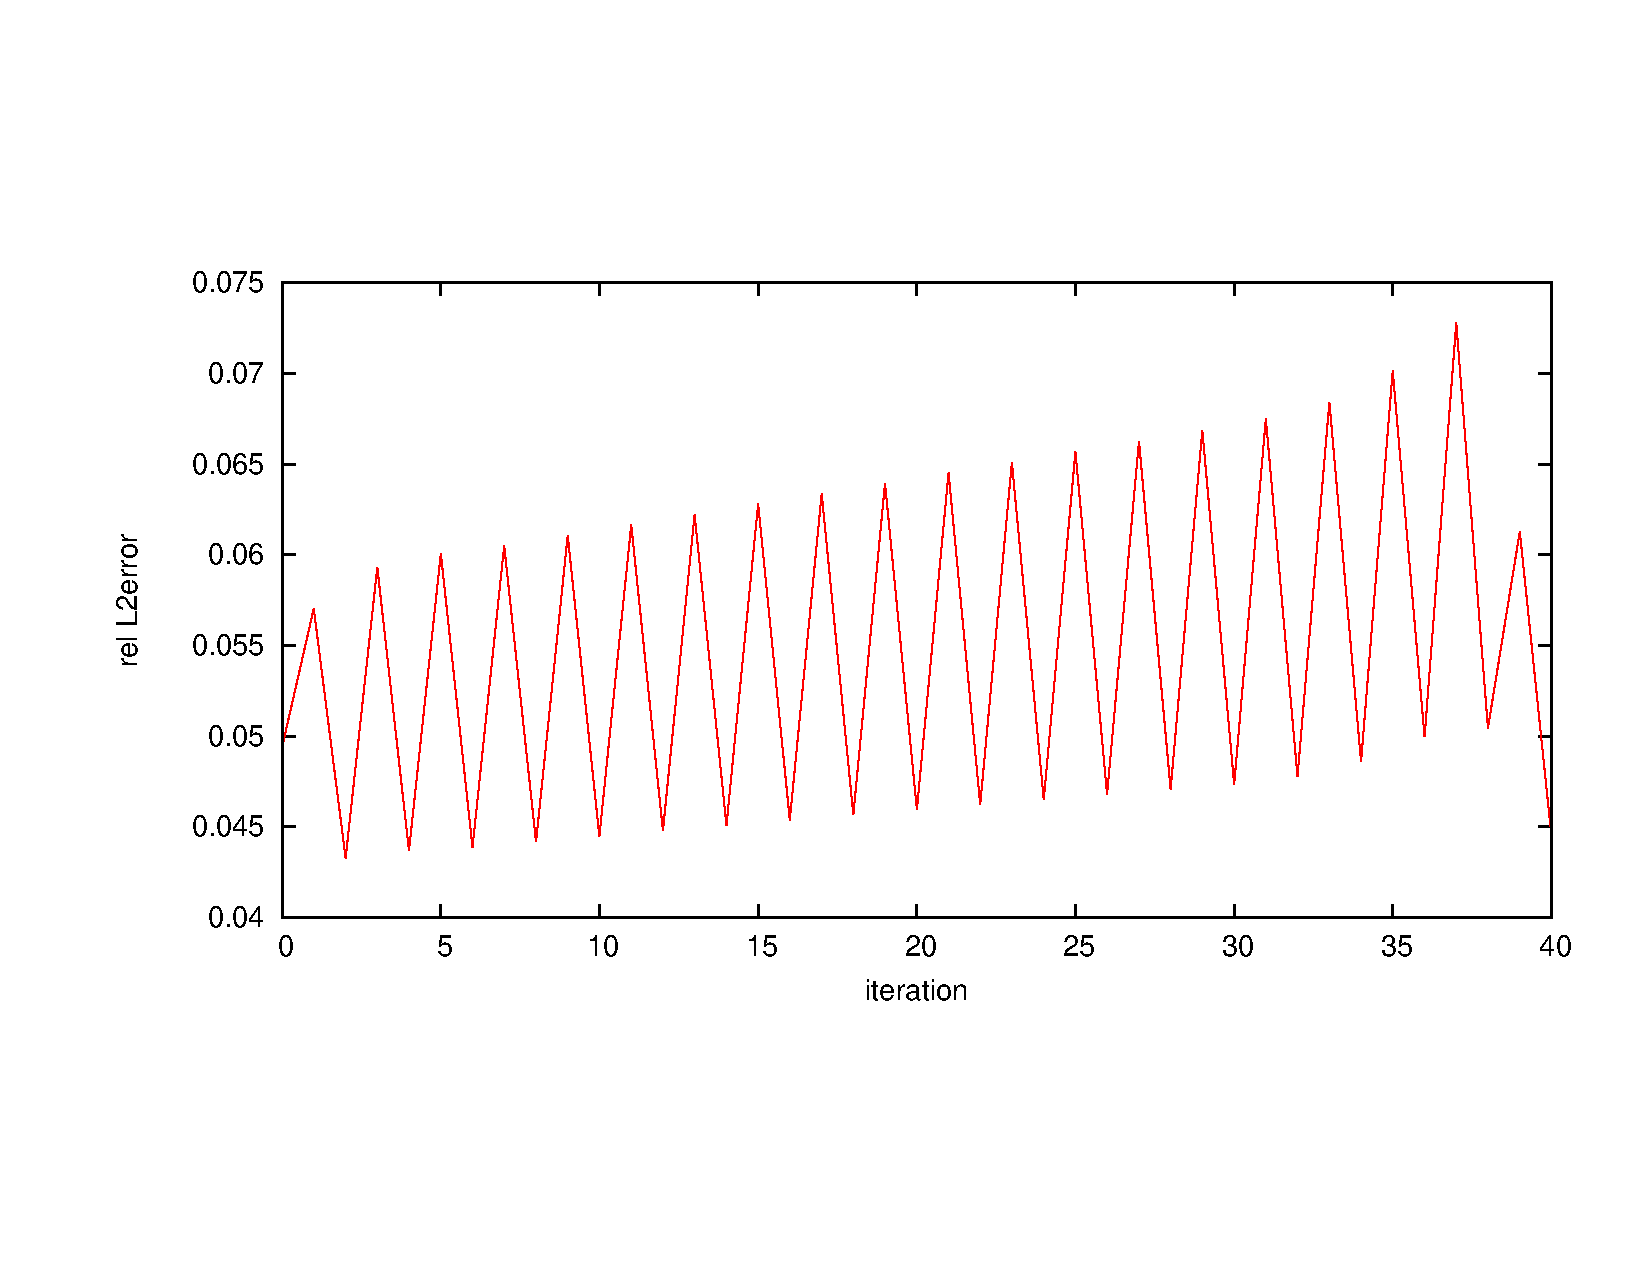
\includegraphics[trim = 2cm 4cm 1cm 4cm, scale=0.5]{plots/oscillation.pdf}
	\caption{Relative $L^2$ error on a grid with $h=\frac 1 4$ and gradient penalty}
	\label{fig: oscillation}
\end{figure}

\begin{figure}[H]
\begin{subfigure}[b]{.5\textwidth}
	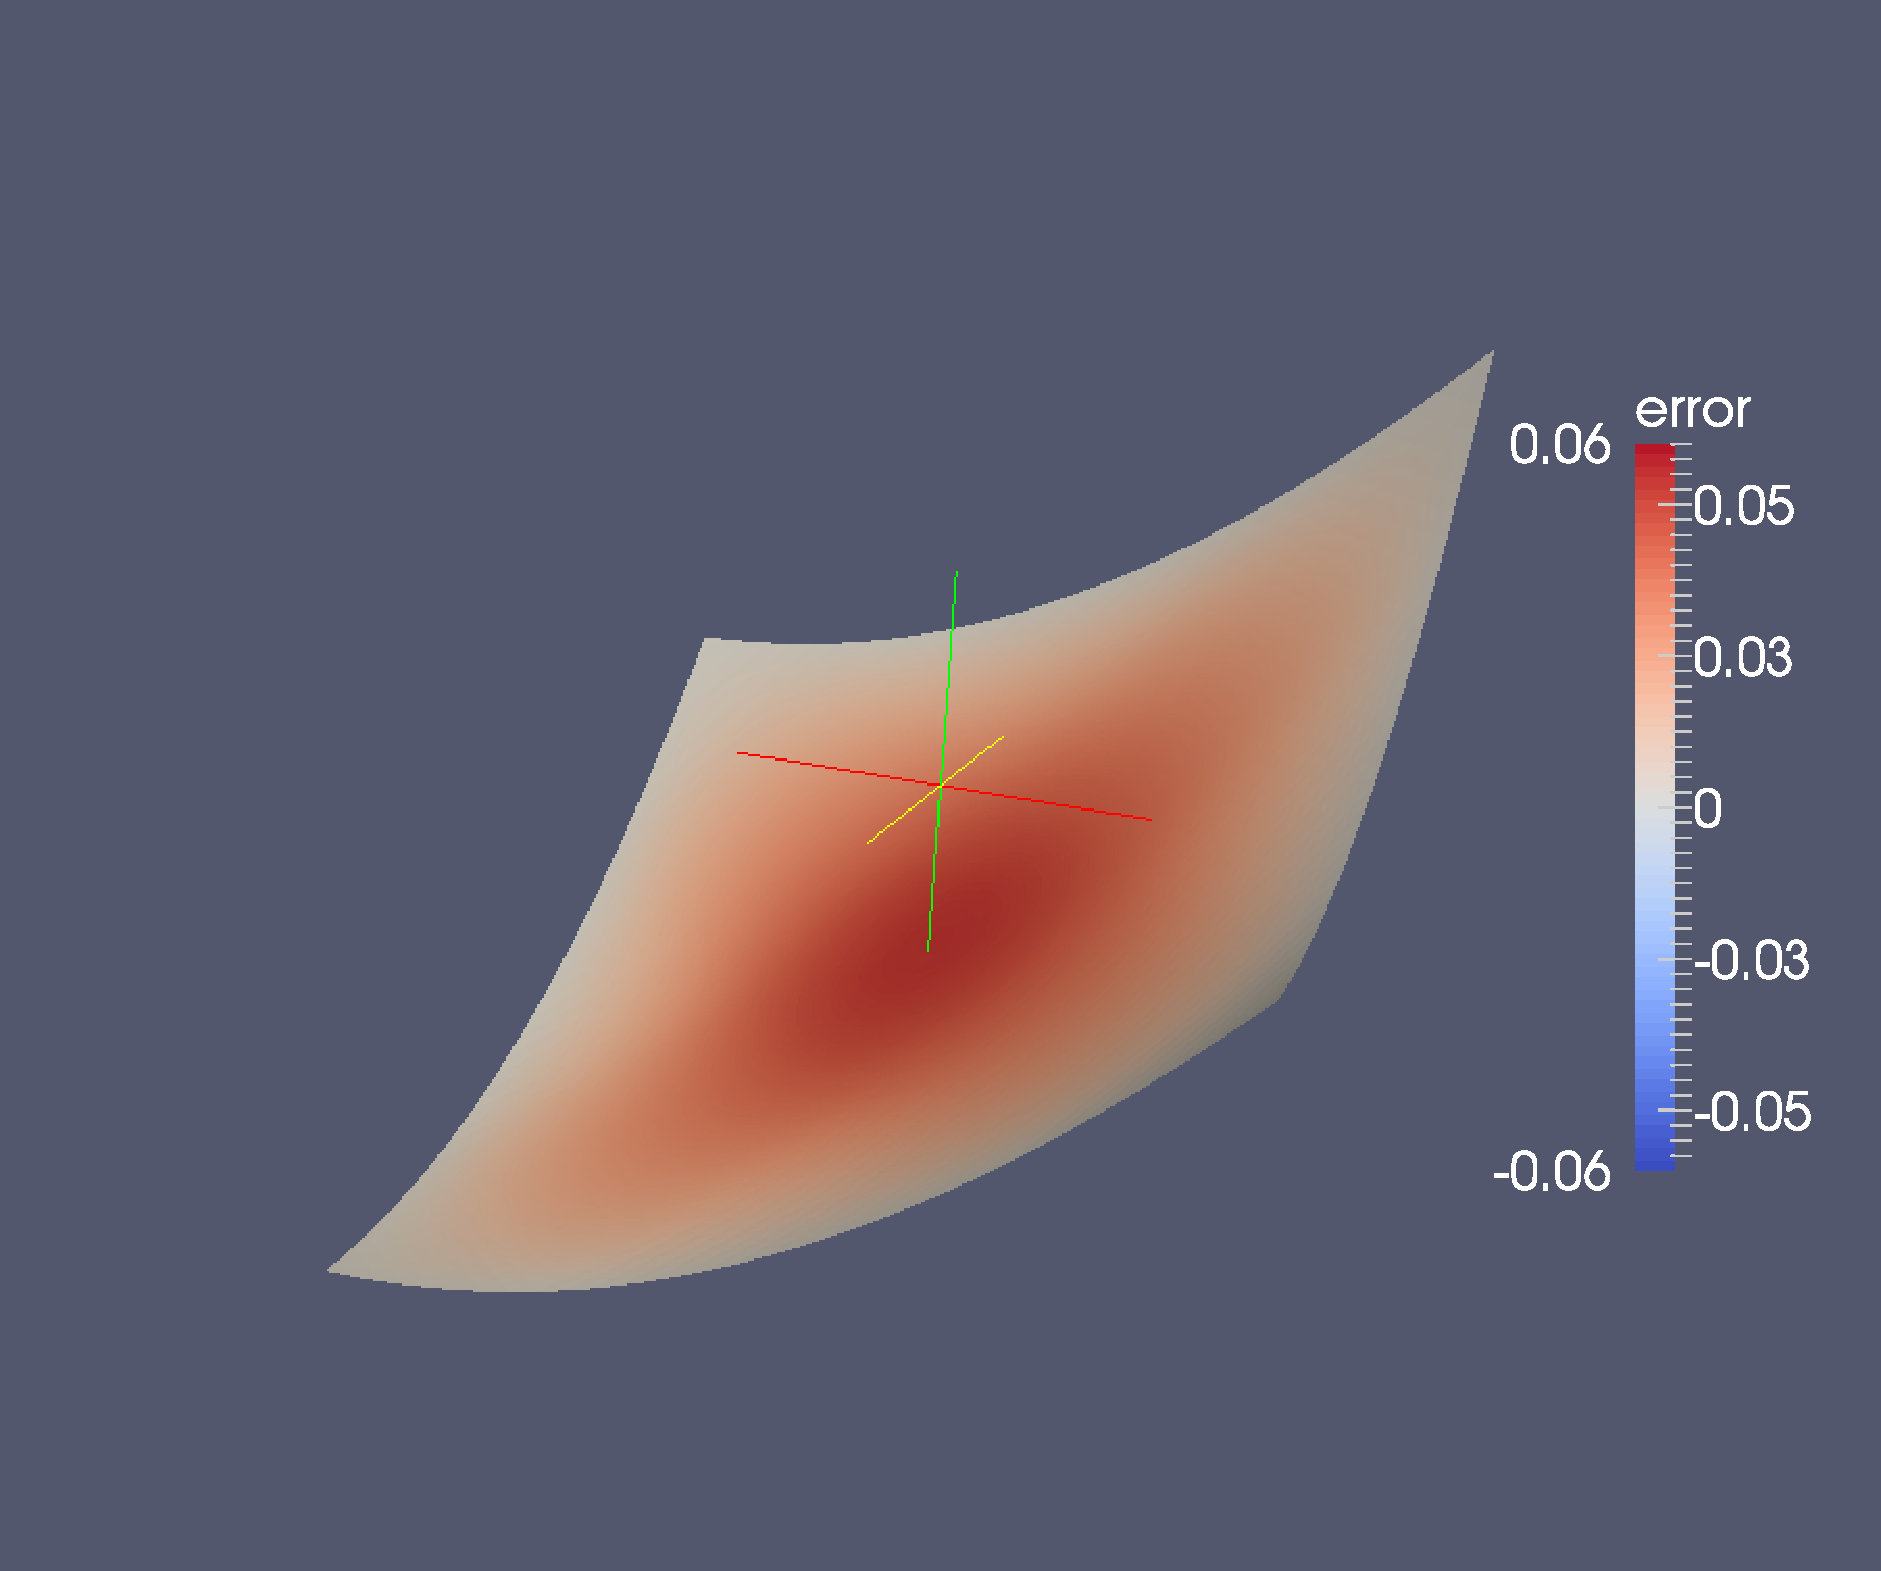
\includegraphics[width=1.\textwidth]{plots/with_penalty_it22.pdf}
	\caption{Solution after 23 steps}
\end{subfigure}
\begin{subfigure}[b]{.5\textwidth}
	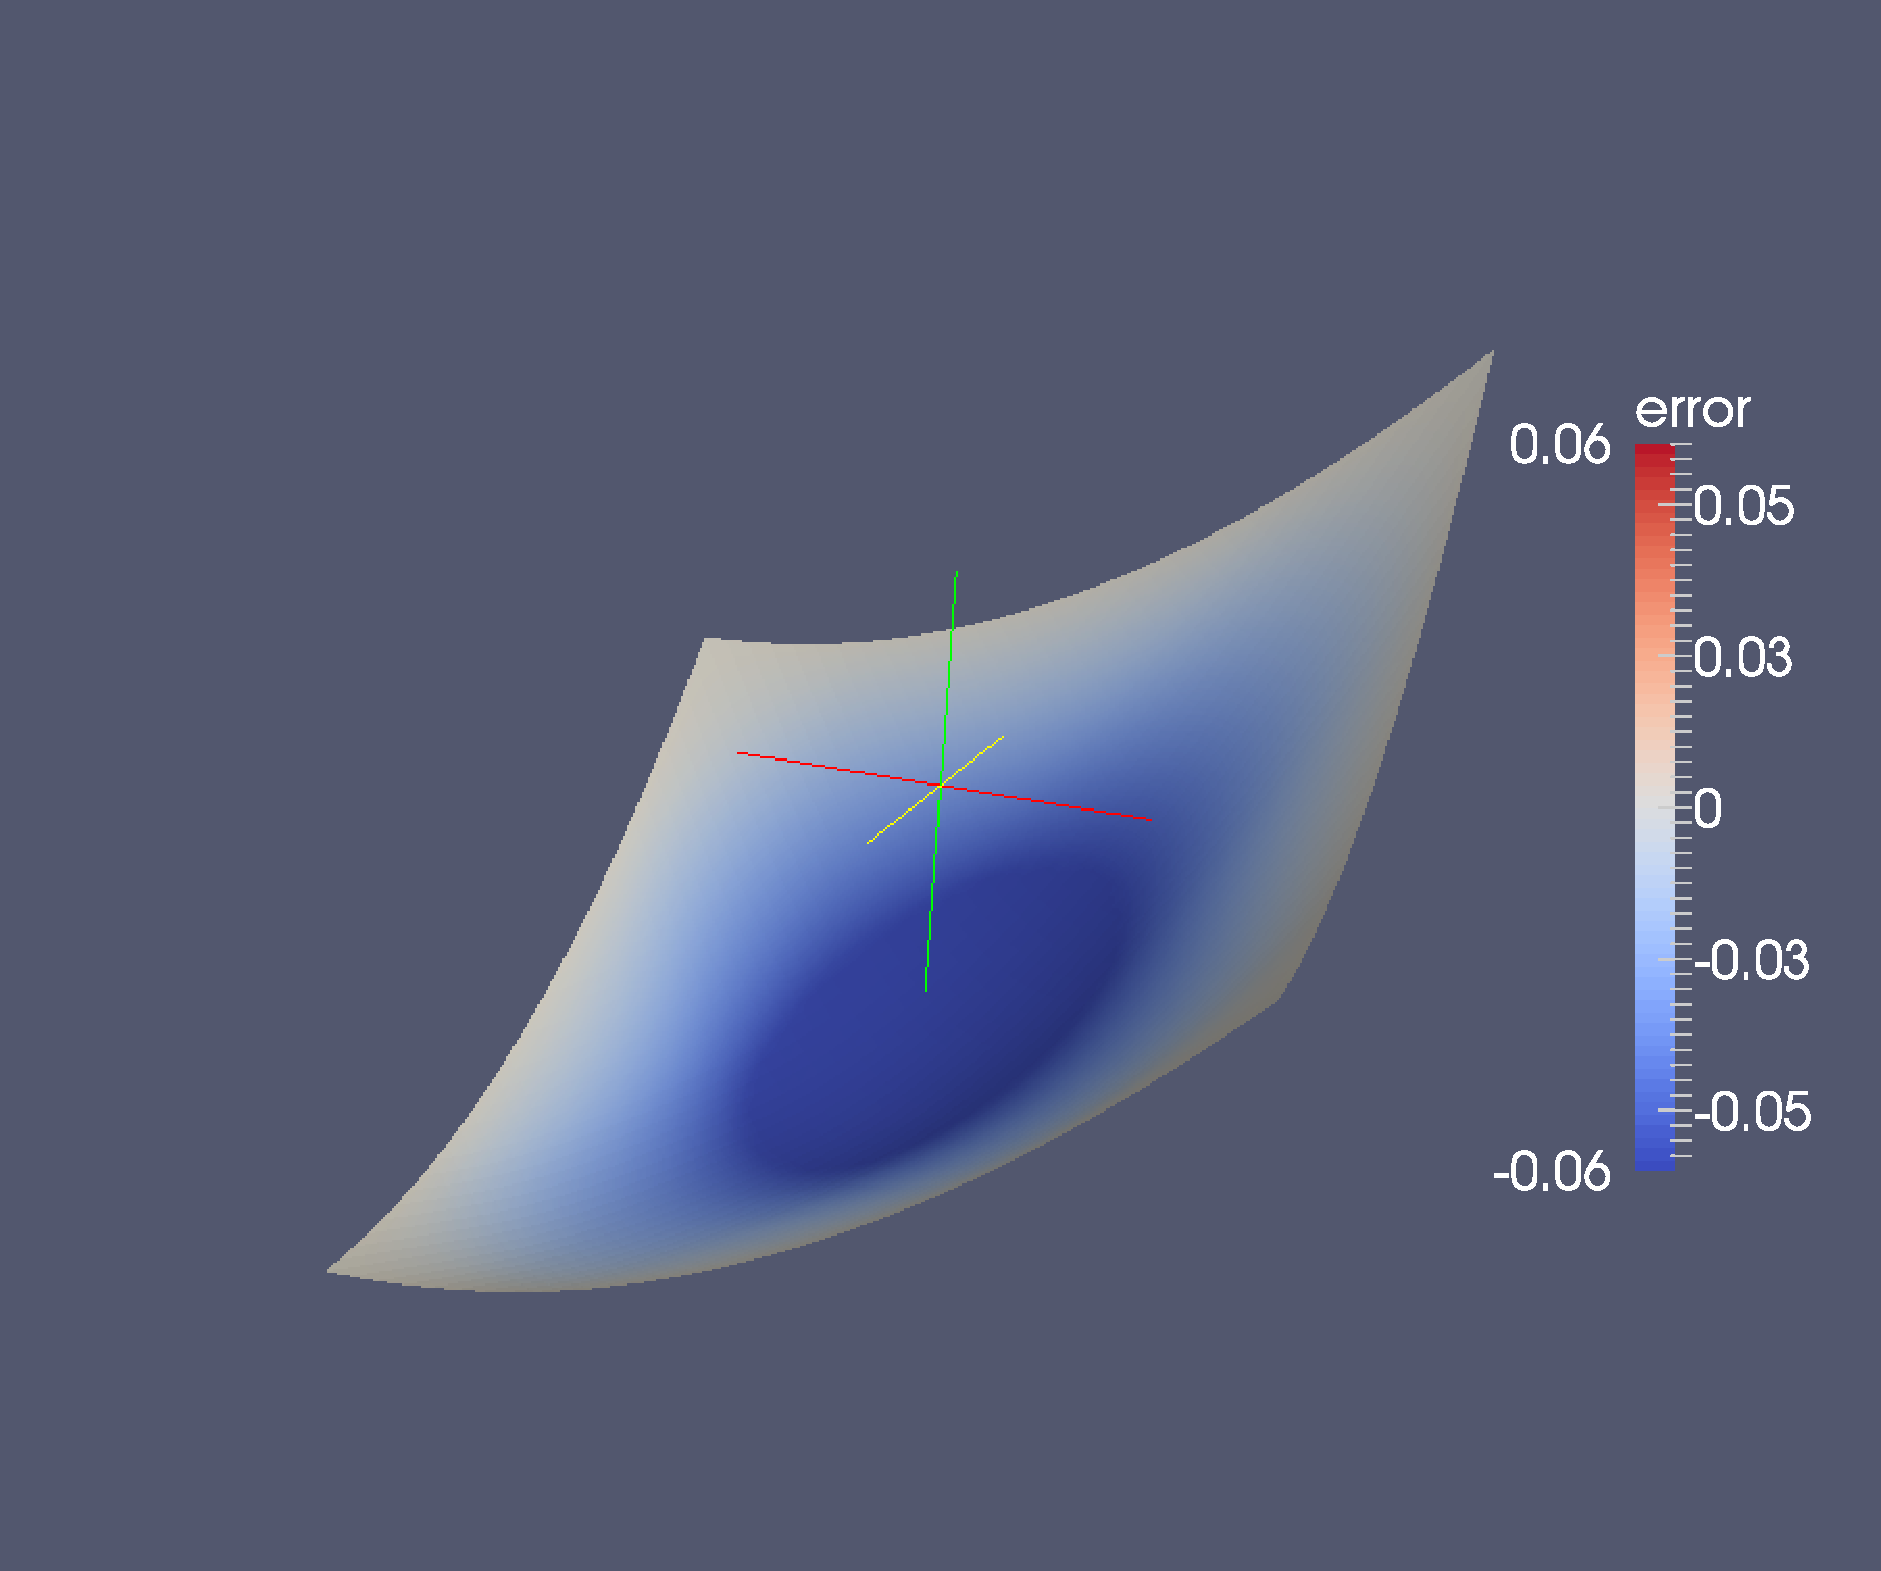
\includegraphics[width=1.\textwidth]{plots/with_penalty_it23.pdf}
	\caption{Solution after 24 steps}
\end{subfigure}
\caption{The solution in two consecutive iterations}
\label{fig: diff iteration}
\end{figure}
Figure \ref{fig: diff iteration} shows two consecutive steps, the error $u-u_{exact}$ is denoted by the surface colour. We see that the solution after 23 steps is mostly red, i.e. it is pointwise greater than the exact solution, while one iteration later the Poisson solution is mostly blue, i.e. it is pointwise smaller than the exact solution. These frames are generic for the behaviour of the intermediate Picard solutions. After a step with a solution $u_h^i$ with $u_h^i \geq u_{exact}$ the solution of the next intermediate function $u^{i+1}_h$ fulfils $u^{i+1}_h \leq u_{exact}$. It looks like the solution is split into two subsequences.  And as we have also seen in the devolution of the error, these subsequences diverge from the exact solution.

%Theoretically it is possible there are two different functions $v,w\in V$ such that $v$ is the solution to the decoupled PDE (cf. \eqref{eq:decoupled PDE}) fixing $w$ and vice versa $w$ the solution of \eqref{eq:decoupled PDE} fixing $v_h$. 
To prevent our algorithm from doing so we couple the two subsequences by a damping. After calculating the new Picard step $u^{i+1}_h$ we combine the current solution with the function calculated one step before by a convex composition $ \alpha u_h^{i+1} + (1- \alpha) u_h^i$ for $\alpha \in (0,1)$. Hence we got a further parameter $\alpha$ to adjust the Picard iteration.

Another parameter sensible to introduce is a parameter to control the ellipticity constant of the used SIPG method.
\subsection{Modification of the Cofactor Matrix}\label{sec: mod cofactor}
For a better ellipticity constant of the Generalised Poisson problem as stated in Section \ref{sec: SIPG MA} it is necessary that the eigenvalues of the diffusion matrix, namely $\mycof{D_h^2 u_h^i}$, are bounded below with some constant $\varepsilon$ (cf. results of Section \ref{sec: SIPG}, in particular Theorem \ref{thm: SIPG stability}).
To fulfil this criterion we add positive multiples of the identity matrix until the smallest eigenvalue becomes $\varepsilon$. Hence, we introduce a modified cofactor matrix
\[ 
	\mycofMod {D^2_h u_h} = \begin{cases}
	\mycof {D^2_h u_h} & \lambda \geq \varepsilon	\\
	\mycof {D^2_h u_h}+ (-\lambda+\varepsilon) Id%\begin{pmatrix} -\lambda+\varepsilon & 0 \\ 0 & -\lambda+\varepsilon \end{pmatrix} 
	& else
	\end{cases}
\]
where $\lambda$ is the minimal eigenvalue of $ \mycof {D^2_h u_h}$ and $Id$ is the $d \times d$-Identity matrix. 
Now we replace all occurrences of $\mycof {D^2_h u_h}$ in \eqref{eq: sipg iteration} by $\mycofMod {D^2_h u_h}$ to stabilise the problem.

The case that a cofactor matrix $\mycof {D^2_h u_h} $ does have a negative eigenvalue or even a complex one implies that also the Hessian of $u_h$ is not positive definite. Hence, $u_h$ is not piecewise convex, we discuss this issue in more detail in the next section.

%Let us recall the geometric interpretation of the second derivative, it indicates the curvature of a function and hence also describes the convexity, concavity respectively.
%One improvement could be the smoothing process during a convexification for it will smooth away all unintended concave curvatures. But probably the result will be still unsatisfiable because convexification does not affect sharp edges at triangle transitions.

\subsection{Convexfication} \label{subsec: convexification}
 The \MA equation in general does not posses a unique solution (cf. Section \ref{sec: Existence and Uniqueness}). Yet for most applications the (unique) convex solution is required. The question is if there exists an appropriate way to oblige the Picard iteration to select only convex solutions.\\
The most intuitive way is to convexify the solution after every step. Thereby, we hope to ensure that the right solution is approximated. There may be additional benefit by a convexification:
Let us recall the geometric interpretation of the second derivative, it indicates the curvature of a function and hence also describes the convexity, concavity respectively. A convexification will smooth away small wiggles and by definition will force the function to be convex.  Thus, a convexification could also improve the approximation quality of second derivatives of our interim solution which we is needed to set up the cofactor of the Hessian for the next Picard step. % aiming for a better approximation of the second derivatives.

Unfortunately convexification is not simple. As there are a lot of results on the convexity of Bernstein polynomials, we choose a Bernstein basis for the ansatz space.
\begin{definition}[Bernstein-B\'ezier form{, \cite[Section.2]{SS2010}}]\label{def: BernsteinBezierForm}
	Any univariate polynomial $p:T \rightarrow \R$ of degree $d$ on a triangle $T$ can be represented in \emph{Bernstein-B\'ezier form} as
\begin{align}
	p(x) = \sum_{\stackrel{i,j,k \in \N}{i+j+k = d}}  c_{ijk} B^d_{ijk}(x),\label{eq: BernsteinBezierForm}
\end{align}
where
\[
	B^d_{ijk}(x) := \frac {d!}{i!j!k!} \beta_1^i \beta_2^j \beta_3^k
\]
are the \emph{Bernstein polynomials} of degree $k$ and $\beta = (\beta_1, \beta_2, \beta_3)\in \R^3$ are the barycentric coordinates of $x \in \R^2$ relative to the triangle $T$.

We call $c=\left(c_{ijk}\right)_{i,j,k \in \N, i+j+k=d}$ also the \emph{B\'ezier coefficents}.
\end{definition}

The B\'ezier coefficients also induce a geometric interpretation. Suppose $T=\langle v_1, v_2, v_3 \rangle$ and the domain points
\begin{align}
	\xi_{ijk} := (i v_1+jv_2 + k v_3) / (i+j+k). \label{eq: domain points}
\end{align} 
Then we call 
\begin{align}
	Q_{ijk} := (\xi_{ijk}, c_{ijk}) \label{eq: control points}
\end{align} the \emph{control points} of a polynomial $p$ defined on $T$. Further we denote the polygon defined by the points $Q_{ijk}$ as the \emph{B\'ezier control polygon}.

\begin{figure}
	\centering
	\usetikzlibrary{calc}
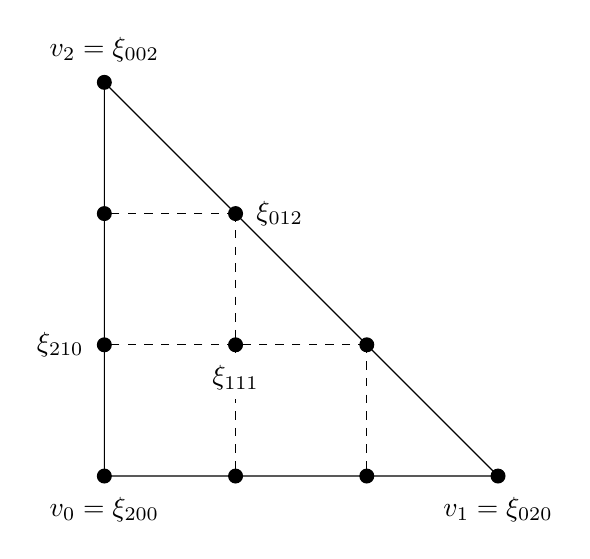
\begin{tikzpicture}[scale=5]

	\draw (0,0) -- (1,0) -- (0,1) -- cycle;

	\edef \n {3}

	\foreach \x in {0,1,...,\n}
{
	\pgfmathtruncatemacro \m {\n -\x}

			\foreach \y in  {0,...,\m}
			{
				\draw [fill]  (\x/\n,\y/\n ) circle [radius=.5pt];
				\if\x 0\else \if \y 0 \else \draw [dashed] (\x/\n,\y/\n ) -- (\x/\n-1/\n,\y/\n); \fi \fi
				\if\y 0\else \if \x 0 \else \draw [dashed] (\x/\n,\y/\n ) -- (\x/\n,\y/\n-1/\n); \fi \fi
			}

}

	\node (v_0) at (0,0)[below=4pt] {$v_0=\xi_{200}$};
	\node (v_1) at (1,0)[below=4pt] {$v_1=\xi_{020}$};
	\node (v_2) at (0,1)[above=4pt] {$v_2=\xi_{002}$};
	
	\pgfmathtruncatemacro \bOne {\n-1}
	\pgfmathtruncatemacro \bTwo {\n-2}
	\node (v_2) at (0,1/\n)[left=4pt] {$\xi_{\bOne 1 0} $};
	\node (v_2) at (1/\n,\bOne/\n)[right=4pt] {$\xi_{0 1 \bOne} $};
	\node[fill=white] (v_2) at (1/\n,1/\n)[below=4pt] {$\xi_{1 1 \bTwo} $};

\end{tikzpicture}
	\caption{The domain points on a triangle $T=\langle v_1, v_2, v_3 \rangle$ for $d=3$}
	\label{fig: domain points}
\end{figure}
Figure \ref{fig: domain points} shows the distribution of the domain points for the polynomial degree $d=3$.

The benefit of the Bernstein-B\'ezier form is that there can be formed simple conditions ensuring the convexity of the polynomial on a triangle. Namely there is a connection between the convexity of the control polygon and the convexity of the polynomial.
\begin{theorem}[ Connection Control Polygon Convexity{\cite[Theorem 4.6]{Dahmen1991}}]
	The convexity of the control polygon implies the convexity of the represented polynomial.
\end{theorem}
Note that this result holds only for a single triangle and not for a function defined on a grid of triangular cells. Nevertheless, piecewise convexity is already very important for the well-posedness of our intermediate SIPG iteration step (cf. Section \ref{sec: SIPG}) such that it is worth a try to convexify the union of all control polygons.

Due to their importance in computer graphics, there are a lot of convex hull algorithm available. Hence it suggests itself to apply a convex hull algorithm on given Bernstein-B\'ezier coefficients to enforce convexity. However, this approach fails for a convex hull algorithm for it only operates on a set of points and hence does not necessarily produce the same connectivity the control polygon implies. An counterexample where those two polygons differ is given in Figure \ref{fig: diff connectivity}:
\begin{figure}[h]
\begin{subfigure}[b]{.5\textwidth}
	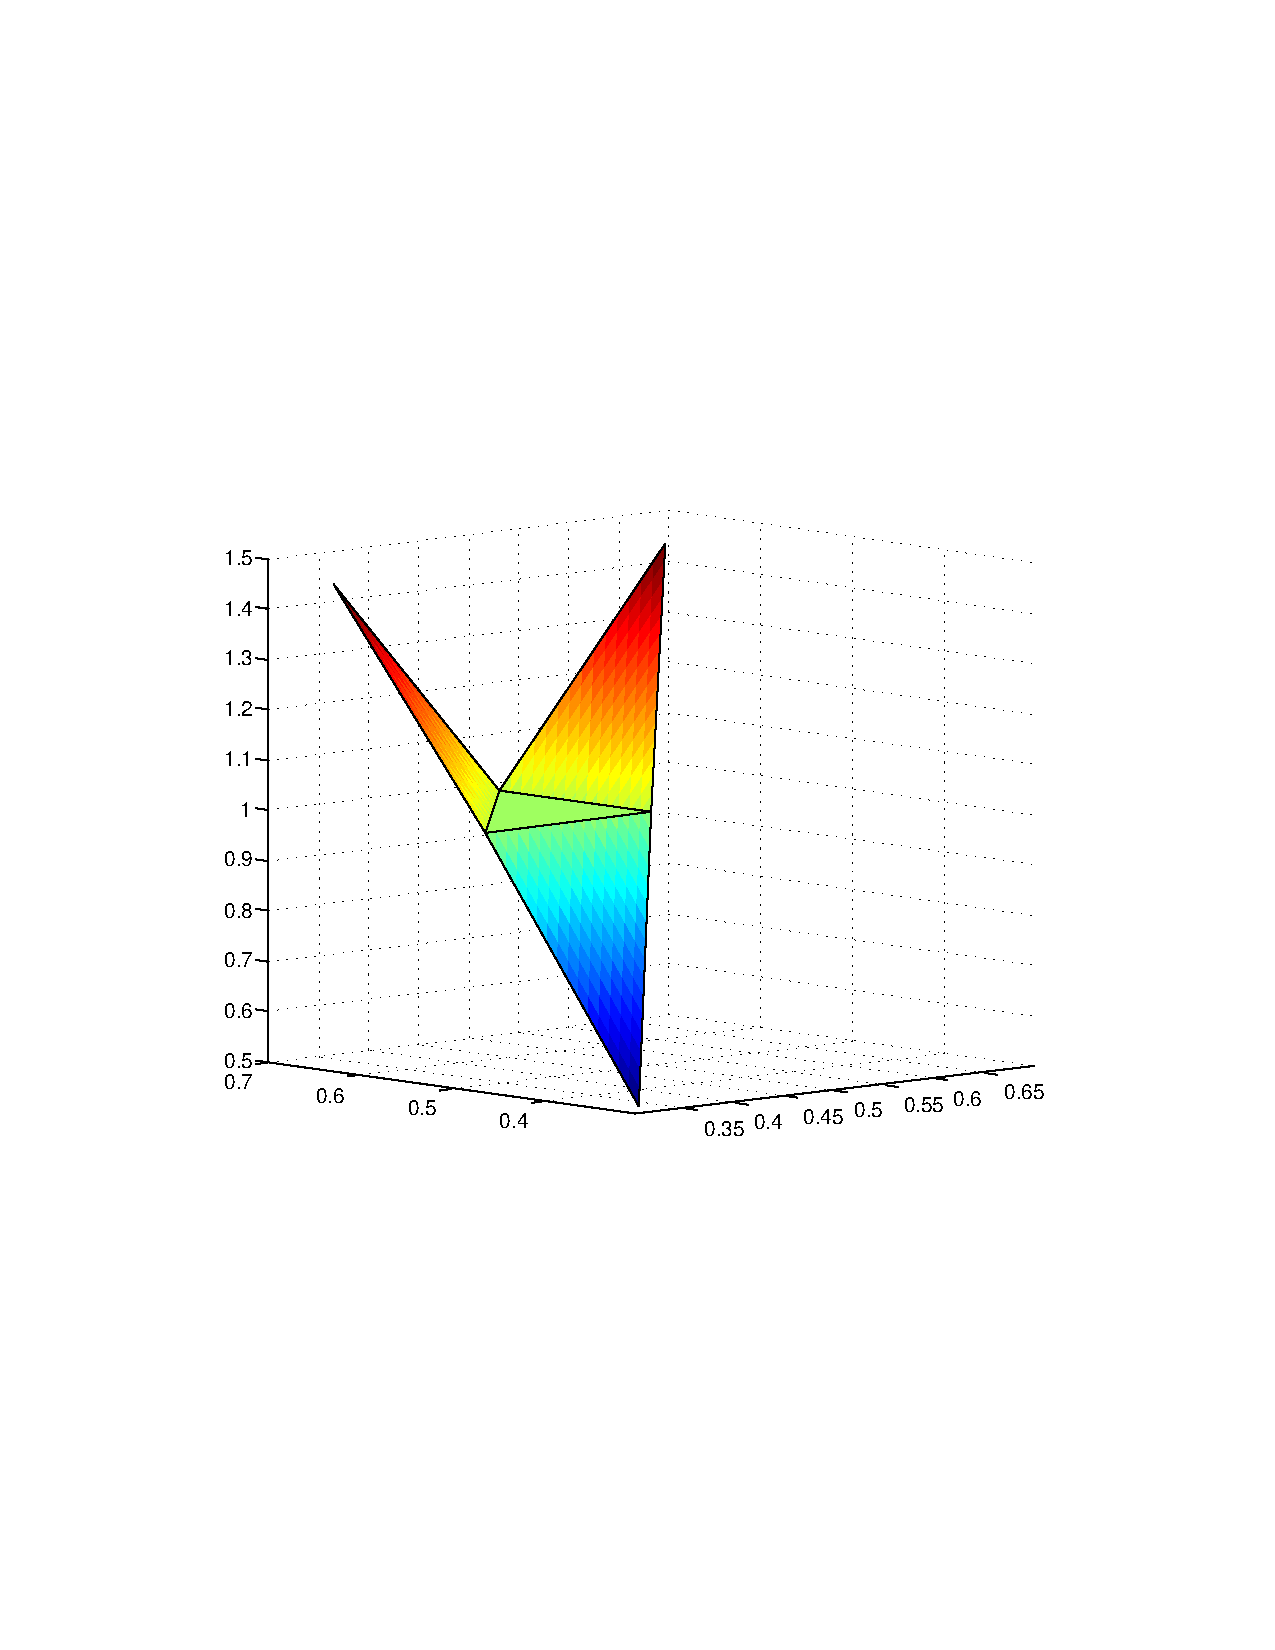
\includegraphics[trim=3cm 8cm 3cm 8cm, width=1.\textwidth]{control_polygon2.pdf}
	\caption{Control polygon}
\end{subfigure}
\begin{subfigure}[b]{.5\textwidth}
	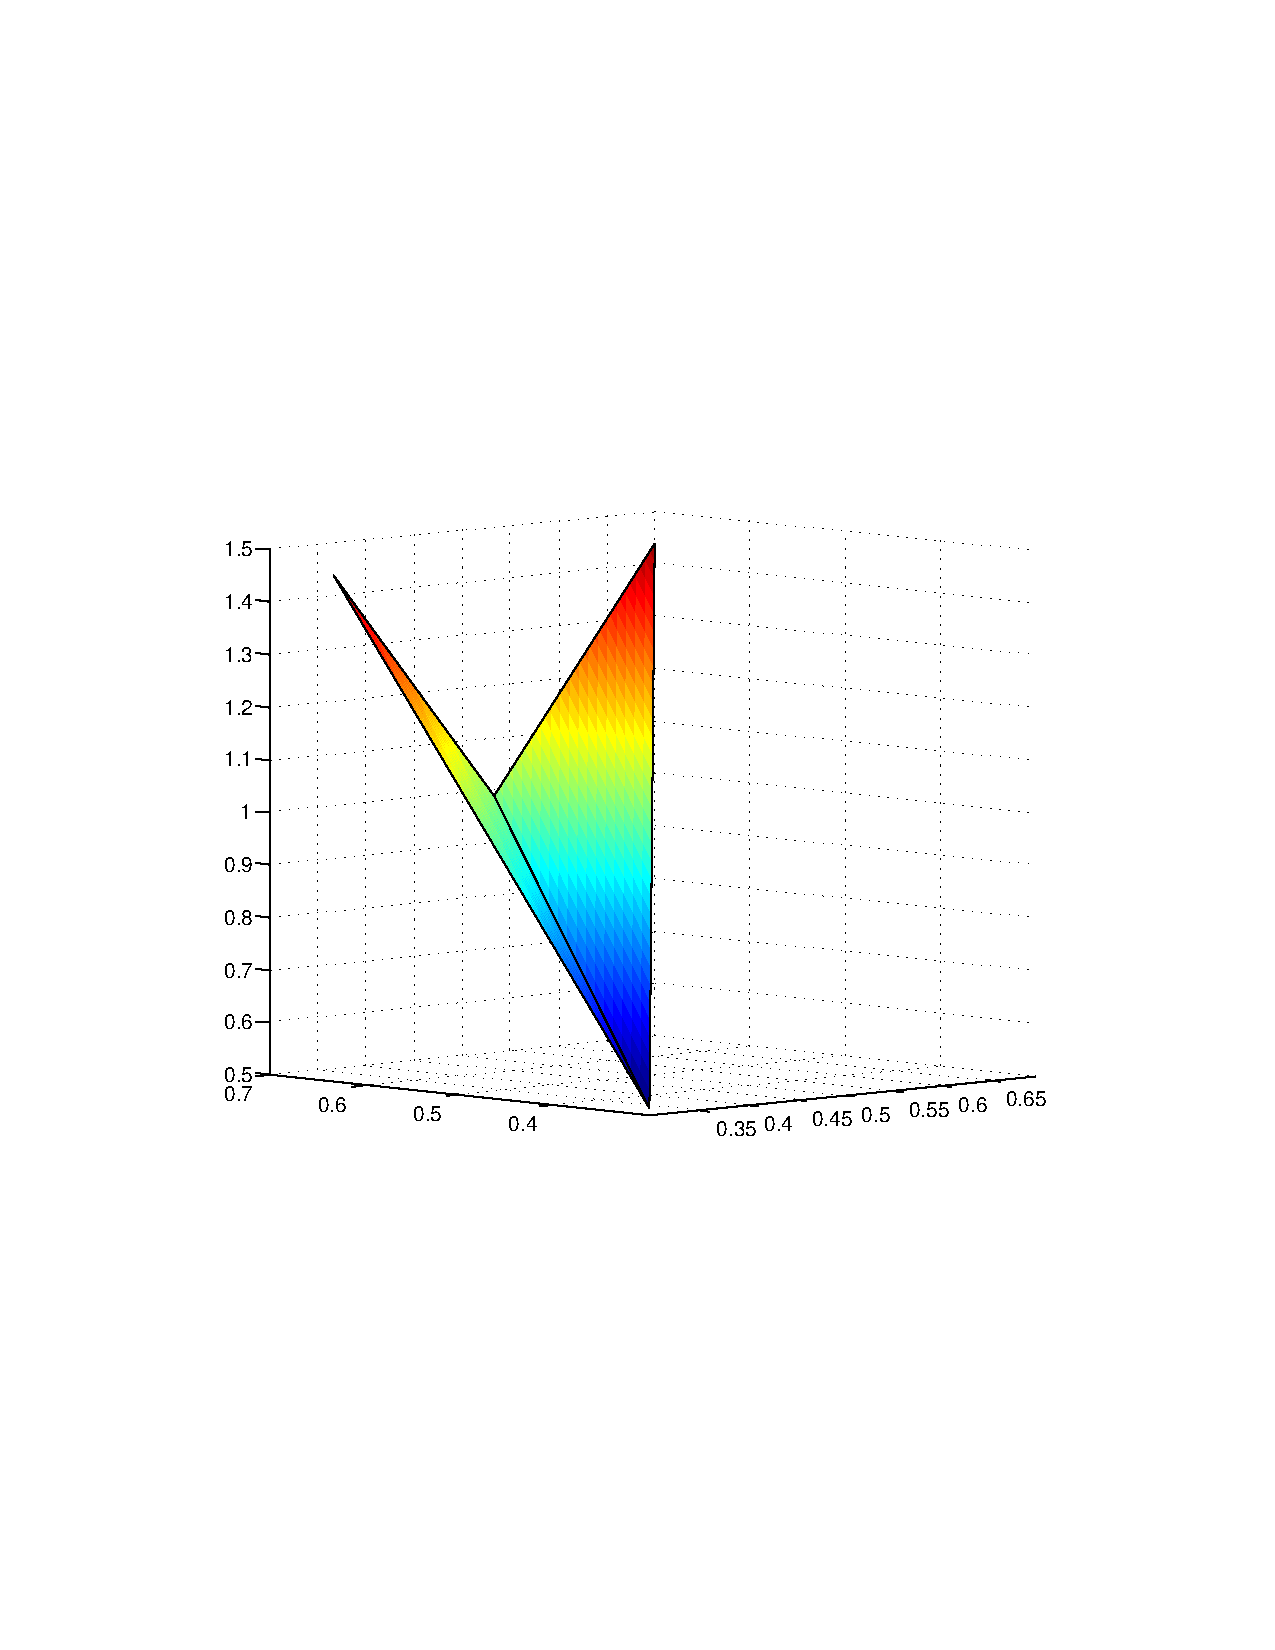
\includegraphics[trim=3cm 8cm 3cm 8cm, width=1.\textwidth]{convex_hull2.pdf}
	\caption{Lower convex hull}
\end{subfigure}
\caption{The control polygon and lower convex hull of a given set of control points}
\label{fig: diff connectivity}
\end{figure}
While the the control polygon is obviously not convex, the surface of the lower convex hull of the control points is convex only because it connects the inner control points differently.

In the eighties mathematicians derived quadratic conditions on the B\'ezier coefficients equivalent to its convexity\cite{CD1984, Dahmen1991}. Later this conditions were relaxed to a set of linear sufficient conditions, yet loosing necessity. To formulate those conditions we use the difference operator $\Delta_{\mu \nu}$ along the edge $(v_\mu, v_\nu)$. 
Thus for the triangle $T=\langle v_1, v_2,v_3 \rangle$ 
%as seen in Figure \ref{fig: domain points} 
we obtain
	\begin{align*}
		\Delta_{21} c_{ijk} &= c_{i,j+1,k} -c_{i+1, j,k}  \\
		\Delta_{31}^2 c_{ijk} &= c_{i,j,k+2} -2c_{i, j+1,k+1} +c_{i, j+2,k} \\
		\Delta_{12} \Delta_{32} c_{ijk} &= c_{i,j+1,k+1} -c_{i+1, j,k+1} - c_{i,j+2,k} +c_{i+1, j+1,k}.
	\end{align*}
 
 For the following theorems  we always refer to the same setting: We have a triangle $T=\langle v_1, v_2,v_3 \rangle$ and a polynomial $p$ of degree $d$ defined on this triangle $T$. Further the B\'ezier coefficents of $p$ are denoted by $c_{ijk}$.
 
A result due to Chang and Feng \cite{CD1984} are the following quadratic constraints.
\begin{theorem}[Convexity on Triangles{\cite[p.2]{LS2007}}] \label{thm: convex cond quadr}
	A polynomial $p$ is convex on a triangle $T$ if and only if the matrix
	\[
		\begin{pmatrix}
			\Delta_{21}^2 c_{ijk} & \Delta_{31} c_{ijk} \Delta_{32} c_{ijk}\\
			\Delta_{31}c_{ijk} \Delta_{32} c_{ijk} & \Delta_{31}^2 c_{ijk} 
		\end{pmatrix} \in \R^2
	\]
	is nonnegative definite for each $i + j + k =d-2 $.
\end{theorem}
For an overview of relaxations of these conditions, we refer to \cite{SS2010}. An example with 12 inequalities is given in the following theorem.
\begin{theorem}[Sufficient Linear Convexity Conditions, {\cite[Corollary 2.8]{SS2010}}]
\label{thm: convex cond on triangle}
	A polynomial $p$ is convex on a triangle $T$ if its B\'ezier coefficients $c_{ijk}$ satisfy
	\begin{align*}
		&(\Delta_{21} + 2\Delta_{31}) \Delta_{31} c_{ijk} \geq 0, 
		&   (\Delta_{21}^2 + 3\Delta_{21} \Delta_{31} + 2 \Delta_{31}^2) c_{ijk} \geq 0, \\
		& \Delta_{21}(2\Delta_{21} + \Delta_{31})  c_{ijk} \geq 0, 
		&   (2\Delta_{21}^2 + 3\Delta_{21} \Delta_{31} +  \Delta_{31}^2) c_{ijk} \geq 0, \\  
		&(\Delta_{32} + 2\Delta_{12}) \Delta_{12} c_{ijk} \geq 0, 
		&   (\Delta_{32}^2 + 3\Delta_{32} \Delta_{12} + 2 \Delta_{12}^2) c_{ijk} \geq 0, \\
		&\Delta_{32} (2\Delta_{32} + \Delta_{12}) c_{ijk} \geq 0, 
		&   (2\Delta_{32}^2 + 3\Delta_{32} \Delta_{12} +  \Delta_{12}^2) c_{ijk} \geq 0, \\  
		&(\Delta_{13} + 2\Delta_{23}) \Delta_{23} c_{ijk} \geq 0, 
		&   (\Delta_{13}^2 + 3\Delta_{13} \Delta_{23} + 2 \Delta_{23}^2) c_{ijk} \geq 0, \\
		& \Delta_{13}(2\Delta_{13} + \Delta_{23})  c_{ijk} \geq 0, 
		&   (2\Delta_{13}^2 + 3\Delta_{13} \Delta_{23} +  \Delta_{23}^2) c_{ijk} \geq 0   
	\end{align*}
	for all $i + j + k = d-2 $.
\end{theorem}
Note that the latter conditions of Theorem \ref{thm: convex cond quadr} and Theorem \ref{thm: convex cond on triangle} ensure convexity on a single triangle $T$. That would suffice for piecewise polynomials contained in $C^1$ because for them, unlike to splines contained in $C^0$ convexity on each triangle implies global convexity \cite[Theorem 3.1.]{SS2010}. To patch this matter Schumaker and Speleers introduce further conditions making sure $C^0$ splines are convex across triangle boundaries in \cite{SS2014}.
\begin{theorem}[Sufficient Conditions across Edges,{ \cite[Theorem 3.6]{SS2014} }]\label{thm: convex cond across edge}
	Let $p \in \mathcal P^d_h \cap C^0(\Omega)$ be a piecewise polynomial being convex on every triangle $T \in \triang$. Suppose its B\'ezier coefficients for every interior edge $e =(v_\kappa, v_\mu)$ fulfil 
	\begin{align}
		{\hat c_{i,j,1}}  \geq  \beta_1^c c_{i+1, 0,j} +\beta_2^c c_{i,1,j} + \beta_1^c c_{i, 0,j+1}, \qquad i+j=d-1, \label{eq: convexity across edge}
	\end{align}
where  $\{c_{i,j,k}\}_{i+j+k=d}$ and $\{ {\hat c_{i,j,k}}\}_{i+j+k=d}$ are the B\'ezier coefficients of $p$ relative to the two triangles $T_1 = \langle v_\kappa, v_\lambda, v_\mu \rangle$ and $T_2 = \langle v_\kappa, v_\mu, v_\nu \rangle$ sharing the edge $e$, and $(\beta_1^c,\beta_2^c,\beta_3^c)$ are the barycentric coordinates of $v_\nu$ with respect to $T_1$. Then $p$ is convex.
\end{theorem}

\begin{figure}[H]
			\begin{center}
		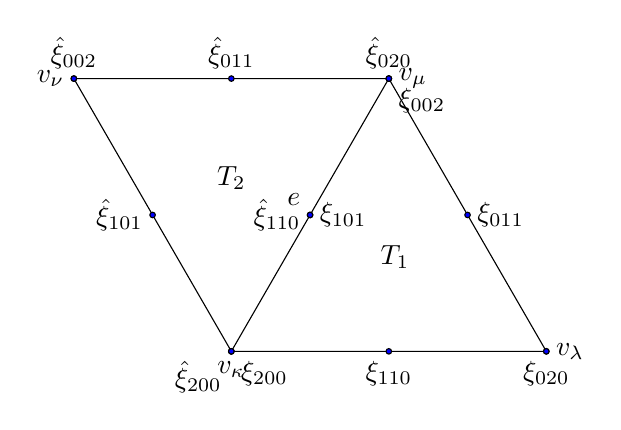
\begin{tikzpicture}
%define coordinates
			\coordinate (vEins) at (120:4cm) ;
			\coordinate (vZwei) at (60:4cm);
			\coordinate (vDrei) at (0:0cm);
			\coordinate (vVier) at (0:4cm);

			\draw (0,0) -- (vEins) -- (vZwei) -- node[above left ] {$e$} (vDrei) -- (vVier) -- (vZwei);

%draw nodes
			\draw[fill =black] (vEins) circle (1pt) node[left] {$ v_\nu$};
			\draw[fill =black] (vZwei) circle (1pt) node[right] {$v_\mu$};
			\draw[fill =black] (vDrei) circle (1pt) node[below] {$v_\kappa$};
			\draw[fill =black] (vVier) circle (1pt) node[right] {$v_\lambda$};

%draw control points in T_1
			\draw[fill =blue] ($(vEins)!0.5!(vZwei)$) circle (1pt) node[above] {$\blue{\hat \xi_{011}}$};
			\draw[fill =blue] ($(vEins)!0.5!(vDrei)$) circle (1pt) node[left] {$\blue{\hat \xi_{101}}$};
			\draw[fill =blue] ($(vDrei)!0.5!(vZwei)$) circle (1pt) node[left] {$\blue{\hat \xi_{110}}$};

			\draw[fill =blue] (vEins) circle (1pt) node[above] {$\blue{\hat \xi_{002}}$};
			\draw[fill =blue] (vZwei) circle (1pt) node[above] {$\blue{\hat \xi_{020}}$};
			\draw[fill =blue] (vDrei) circle (1pt) node[below left] {$\blue{\hat \xi_{200}}$};

%draw control points in T_2
			\draw[fill =blue] ($(vVier)!0.5!(vZwei)$) circle (1pt) node [right] {$\blue{\xi_{011}}$};
			\draw[fill =blue] ($(vVier)!0.5!(vDrei)$) circle (1pt) node[below] {$\blue{\xi_{110}}$};
			\draw[fill =blue] ($(vDrei)!0.5!(vZwei)$) circle (1pt) node[right] {$\blue{ \xi_{101}}$};

			\draw[fill =blue] (vZwei) circle (1pt) node[below right] {$\blue{\xi_{002}}$};
			\draw[fill =blue] (vDrei) circle (1pt) node[below right] {$\blue{\xi_{200}}$};
			\draw[fill =blue] (vVier) circle (1pt) node[below] {$\blue{ \xi_{020}}$};

			\draw node at (90:2.2cm) {$T_2$};
			\draw node at (30:2.4cm) {$T_1$};
			
		\end{tikzpicture}
		\end{center}

	\caption{Two triangles and B\'ezier control points for polynomials of degree $k=2$ \\($T_1 = \langle v_\kappa, v_\lambda, v_\mu \rangle$ and $T_2 = \langle v_\kappa, v_\mu, v_\nu \rangle$)}
	\label{fig: convexity condition}
\end{figure}
Figure \ref{fig: convexity condition} shows the domain points $\xi_{ijk}$ (cf. \eqref{eq: domain points}) corresponding to the B\'ezier coefficients of the scenario of Theorem \ref{thm: convex cond across edge} for the case $d=2$.

 Let us consider the condition
\[
		{\hat c_{101}} \geq \beta_1^c c_{200} +\beta_2^c c_{110} + \beta_1^c c_{101}	
\]
Geometrically in the case of $d=2$ this ensures the control point $Q_{101}$ (cf. \eqref{eq: control points})is above the plane where the triangle $\langle Q_{200}, Q_{110}, Q_{101} \rangle$ is embedded. %Note that the first two coordinates are the coordinates of the domain points. Thus, we can identify the 
Or in particular the surface consisting of the triangle $\langle Q_{200}, Q_{110}, Q_{101} \rangle= \langle \hat Q_{200}, Q_{110}, \hat Q_{110} \rangle$  and the triangle $\langle \hat Q_{200}, \hat Q_{110}, \hat Q_{101} \rangle$ is convex.

For quadratic splines Schumaker and Speleers prove the inversion of Theorem \ref{thm: convex cond across edge} on convex domains $\Omega$, namely if for every interior edge its coefficients satisfy \eqref{eq: convexity across edge} then the corresponding spline is convex \cite[Corollary 3.10]{SS2014}.
This result does not generalise for higher degrees. In fact they give a counterexample for degree $k = 3$ \cite[Example 3.11]{SS2014}.

Now we apply the new insights to the solution of the Generalised Poisson problem stated in Section \ref{sec: SIPG MA}.
Given the DG solution of the Generalised Poisson problem $u^{gp}_h$ we seek for a convex spline minimising the error at the B\'ezier control points, i.e. we want to find the B\'ezier coefficients $c$ minimising
\begin{align}
		\lVert A c - b \rVert_2, \qquad \text{ such that } Cc \geq 0, \label{eq: convex lsq}
\end{align}
where $A$ is the matrix evaluating the piecewise polynomial induced by the B\'ezier coefficients $c$ corresponding  at the domain points (cf. \eqref{eq: domain points}), $b$ are the function values of $u^{gp}_h$ at the B\'ezier control points and $C$ is the matrix containing the conditions ensuring convexity on the whole domain.

However, solving a linearly constrained least squares problem is nontrivial. So, when using this approach one should ensure that a convexification is justified. Also, one has to keep in mind that the constraints in the matrix $C$ are sufficient but not necessary. We discuss in Chapter \ref{ch:NumericalResults} whether this approach fulfils our requirements on a convexificiation.

\section{The Picard Iteration Algorithm} \label{sec: Picard Iteration Algo}

Combining the suggestions of the last sections we obtain a method to carry out the fixed point iteration working as Algorithm \ref{alg: final} describes.

\begin{algorithm}[H]
\begin{algorithmic}
\Require triangulation \triang, desired mesh width $h$, maximimal number of intermediate steps $i_{max}$
\State $u_0\gets $ solution of  $
	\triangle u = \sqrt{2f} \text{ in } \Omega $ with $
	u = g \text{ on }\partial \Omega$ \Comment initialisation
\While {$h < H$}
	\State $i \gets 0$
%	\While {$|u_i-u_{i-1}| < \varepsilon$}
	\While {$i < i_{max} $}
		\State $u_i \gets$ solution of \ref{sec: SIPG} with modified cofactor matrix (\ref{sec: mod cofactor})
		\State (convexify)
		\State $u_i \gets \alpha u_{i-1} + (1-\alpha)u_i $ \Comment convex combination
		\State $i \gets i+1$
	\EndWhile
	\State $h, \triang \gets h/2, \triangFine$
\EndWhile
\end{algorithmic}
\caption{Picard Iteration Algorithm to Solve the \MA Equation}
\label{alg: final}
\end{algorithm}

The step convexify is put into brackets for it is not clear whether a convexification is necessary and actually helps the convergence. A lot of the methods mentioned in the Chapters \ref{ch:MongeAmpereEq} and \ref{ch:DGMongeAmpere} work without an explicit convexification, although most require a convex initial guess. 
Additionally the approach described in Section \ref{subsec: convexification} is intricately to implement, significantly increases the computation costs and may modify functions even though they already are convex. We note, that for the well-posedness of the used SIPG method we need the cofactor matrix to be positive definite which is equivalent to the piecewise convexity of the last iteration step. However, our modification of the cofactor matrix  may avert the problems arising for slightly non-convex intermediate solutions.
